%%%%%%%%%%%%%%%%%%%%%%%%%%%%%%%%%
%Preamble
%%%%%%%%%%%%%%%%%%%%%%%%%%%%%%%%%

\PassOptionsToPackage{usenames, dvipsnames}{xcolor}

\documentclass[11pt, a4paper, table]{article}
\usepackage[english]{babel}
\usepackage[margin=1in]{geometry}
\usepackage[ruled, vlined]{algorithm2e}

\usepackage{amsfonts}
\usepackage{setspace,graphicx,epstopdf,amsmath}
\usepackage{marginnote, datetime, url, enumitem, subfigure}
\usepackage[capposition=top]{floatrow}

%Journal Style
%JFE looks nice, JF looks awful
	\usepackage{amsthm}
	\usepackage{jfe}

%Bibliography Stuff
	%Use natbib even though it's old because it's compliant with journal styles
	%Actual bibliography style etc are specified where you actually want it
	\usepackage{natbib}

%Fluff
	\linespread{1.3}

%Neural Network Packages
	\usepackage{neuralnetwork}
	\usepackage{xpatch}
	\makeatletter
	% \linklayers have \nn@lastnode instead of \lastnode,
	% patch it to replace the former with the latter, and similar for thisnode
	\xpatchcmd{\linklayers}{\nn@lastnode}{\lastnode}{}{}
	\xpatchcmd{\linklayers}{\nn@thisnode}{\thisnode}{}{}
	\makeatother
	
%Regression Tree
	\usepackage{tikz,forest}
	\usetikzlibrary{arrows.meta}
	
	\forestset{
		.style={
			for tree={
				base=bottom,
				child anchor=north,
				align=center,
				s sep+=1cm,
				straight edge/.style={
					edge path={\noexpand\path[\forestoption{edge},thick,-{Latex}] 
						(!u.parent anchor) -- (.child anchor);}
				},
				if n children={0}
				{tier=word, draw, thick, rectangle}
				{draw, diamond, thick, aspect=2},
				if n=1{%
					edge path={\noexpand\path[\forestoption{edge},thick,-{Latex}] 
						(!u.parent anchor) -| (.child anchor) node[pos=.2, above] {Y};}
				}{
					edge path={\noexpand\path[\forestoption{edge},thick,-{Latex}] 
						(!u.parent anchor) -| (.child anchor) node[pos=.2, above] {N};}
				}
			}
		}
	}

\usepackage{lscape}
\usepackage{longtable}

%%TODONOTE commands
\usepackage[colorinlistoftodos]{todonotes}
\newcommand{\smalltodo}[2][] {\todo[caption={#2}, size=\scriptsize,%
	fancyline,#1]{\begin{spacing}{.5}#2\end{spacing}}}
\newcommand{\rhs}[2][]{\smalltodo[color=green!30,#1]{{\bf RS:} #2}}
%%

%Graphs
\usepackage{tikz}
\usepackage{pgfplots}
\usepackage[export]{adjustbox}

\graphicspath{{../Results/}}

%Coloured Tables

%%%%%%%%%%%%%%%%%%%%%%%%%%%%%%
%%Title and other fluff, just before document start
%%%%%%%%%%%%%%%%%%%%%%%%%%%%%%

%Hyperref apparently is a big package and causes a lot of issues, so it's recommended to load this last

\usepackage{hyperref}

%Gets rid of the neon green boxes around boxes

\usepackage[]{xcolor}

\hypersetup{
	colorlinks,
	linkcolor = {red!50!black},
	citecolor = {blue!50!black},
	urlcolor = {blue!80!black}
}

\title{Evaluation of Machine Learning in Empirical Asset Pricing
\thanks{I acknowledge and thank David Frazier, my supervisor, Xueyan Zhao and Jun Sung Kim, my honours degree coordinators, as well as my fellow honours cohort for their support throughout the writing of this thesis. I would also like to acknowledge the work of \cite{gu_empirical_2018}, and in particular for their provision of the dataset which they constructed.}
}
\author{Ze Yu Zhong \\
Supervisor: David Frazier \\ 
Thesis submitted for the completion of the \\
Bachelor of Commerce (Honours) in Econometrics at \\
Monash University}

%%%%%%%%%%%%%%%%%%%%%%%%%%%%%%%
%%BEGIN DOCUMENT
%%%%%%%%%%%%%%%%%%%%%%%%%%%%%%%

\begin{document}

\maketitle

\begin{abstract}
We explore the performance of some common machine learning algorithms in empirical asset pricing with regards to prediction performance and causal inference through a simulation study and empirical study, with special focus on how well they deal with the stylized facts and problems in financial returns data. We evaluate prediction performance according to MSE, MAE and out-of-sample R-Squared, and factor significance assessed using a variable importance metric. Across both the simulation and empirical, we find consistent results that contradict those documented in the literature, and conclude that elastic net models perform the best both in terms of prediction performance and causal ability, followed by random forest models. We take particular note that neural networks fail to outperform other machine learning models, and highlight their non-robustness. Almost all machine learning models considered outperformed traditional regression by a large margin, and we show that machine learning methods offers some potential tools for the field of empirical finance. 
\end{abstract}

\newpage

\tableofcontents

\newpage

%%%%%%%%%%%%%%%%%%%%%%%%%%%%%%%%%%%%%%%%%%%%%%%%%%%%%%%%%%%%%%%%%%%%%%%%%%%%%%%%%%%%%%%%%%%%%%%%%%%%%

\section{Introduction}

\subsection{Topic}

This thesis aims to evaluate the application of machine learning algorithms in empirical asset pricing. While there has been significant recent interest in applying machine learning to the problem of predicting asset returns, there is little literature that focuses on how well these methods perform in terms of prediction and variable importance influence when applied to datasets which exhibit the characteristics, or ``stylized facts" of empirical returns. Two studies were conducted to explore this: simulation study consisting of  simulated datasets ranging from linear to highly non-linear data generating processes incorporating observed phenomena and of cross sectional correlation, persistence, and stochastic volatility, and an empirical study using real world data. We focus our study on four popular and representative machine learning models: linear models, elastic net models, random forests and neural networks. Model performance is assessed according to their predictive performance, measured by Mean Absolute Error, Mean Squared Error, and Predictive $R^2$, and their ability at conducting factor significance, as measured by a variable importance metric.

\subsection{Background Literature and Motivations}

Empirical finance can be broadly classified into two main fields: improving the prediction of future excess returns, and understanding the underlying relationship\footnote{We avoid using the terminology of ``causal" relationship because of the difficulty in defining causality in the context of time series, though note the sporadic use of this term in the literature (see \cite{lee_causal_1992} and \cite{hameed_time-varying_1997}).} among factors that drive excess returns. These two goals are noted to be very challenging for traditional regression methods, and this is largely due to the challenges present in the variables that affect financial data, also known as ``factors." 

We define ``factors" with the more contemporary definition as suggested by \cite{harvey__2016}: a collection of regressors to be used in pricing excess returns that can be used to proxy for unknown underlying risk factors due to their correlation with cross sectional returns. \footnote{Most notably, their definition rejects the more strict view that risk factors should be variables that have unpredictable variation through time, and that they should be able explain cross sectional return patterns.} \cite{harvey__2016} further group factors into the two broad categories of ``common" and individual firm ``characteristics." ``Common" factors under this definition can be viewed as proxies for sources of risk constant across all firms, such as macroeconomic variables. Examples of this include the Fama-French factors, which are excess returns on portfolios of assets sorted by certain characteristics to proxy for them. 

Because of this less strict definition factors are often noted for exhibiting properties which make them highly unsuitable for inclusion in traditional regression, (\cite{harvey__2016}). Factors have been empirically observed to have high persistence, high cross-sectional correlation (multicollinearity), non-stationarity or low time series variation due to being pre-known or suffering from a lower sampling frequency. The consequences of including such regressors into traditional regression models are well documented. The resulting coefficient estimates and t-statistics can be biased, directly leading to incorrect statistical inference. Additionally, the variances for the coefficient estimates can be very high, resulting in imprecise coefficient estimates. Any subsequent out of sample predictions from these models, which are a direct function of these imprecise coefficients, also imprecise, particularly when the multicollinearity between variables changes over time, resulting in poor prediction performance.

Several real world examples of this behaviour have been documented in the literature, and perhaps the most infamous examples are the dividend ratio factors. Dividend ratio factors were initially very popular in the 1990s due to its inclusion in regression improving in sample performance. However, later literature such as \cite{goetzmann_testing_1993} and \cite{ang_stock_2006} note the persistence present in dividend ratio factors. This means that movements in dividend ratios are dominated by movements in price and therefore dividend ratios are correlated with lagged dependent variables on the right hand side of the regression equation. This violates the assumptions of exogeneous regressors (independent from the error term) required for traditional regression models (ordinary least squares) to be unbiased, resulting in t-statistics which are biased upwards and increase with time horizon due to autocorrelated errors. Importantly, \cite{goetzmann_testing_1993} show that corrections to t-statistics using the Generalized Method of Moments and Newey-West standard errors also appear to be biased upwards, making them unreliable. 

\cite{goyal_predicting_2003} provide a more comprehensive study on the performance of lagged dividend price ratios, with a specific focus on out of sample predictive performance both in terms of $R^2$ and forecast errors. They conclude that while models incorporating dividend related factors were able to achieve higher in sample performance prior to 1990 than the historical mean, they could not have outperformed the historical mean \textit{out of sample}. \cite{goyal_predicting_2003} attribute this to the increasing persistence and non-stationarity of dividend ratios, noting that they have become like random walks as of 2001. This mirrors the sentiment of (\cite{lettau_consumption_2001}, \cite{schwert_anomalies_2003} and others) who conclude that models incorporating dividend ratios seemed to break down in the 2000s due to a changing economic environment, despite having performed well in the 1990s.

Despite the controversy, the prevailing tone within the literature was that various factors such as dividend ratios, earnings price ratio, interest and inflation and other financial indicators were able to predict excess returns, with \cite{lettau_consumption_2001} remarking that this was now ``widely accepted." However, \cite{welch_comprehensive_2008} extend the work of \cite{goyal_predicting_2003} by including a more comprehensive set of variables and time horizons. They conclude that not a single variable had any statistically significant forecasting power. Crucially, they demonstrate the non-robustness of models incorporating these factors by showing that the significance values of some factors change with the choice of sample periods.

Despite this, the literature has continued to produce more factors: quantitative trading firms were using 81 factor models as the norm by 2014 \citep{hsu_finding_2014}, and \cite{harvey_census_2019} currently document well over 600 different factors suggested in the literature. 

The dramatic increase in the number of factors alone poses challenges to traditional statistical techniques. \cite{harvey__2016} detail the false discovery problem when the number of potential factors is extremely high. The significance of a factor in a traditional regression setting is determined by a single hypothesis test, which by construction carries a level of significance $\alpha$ controlling the type I error rate: the probability of rejecting a "null" hypothesis that a factor is not important, and concluding that it is significant when the true factor is indeed insignificant. When the number of potential factors is large, it is much more likely that a factor will be concluded as significant by pure chance. For example, a factor model consisting of 600 factors would find around 30 factors significant by chance at the 5\% significance level. \cite{harvey__2016} produce a multiple testing framework to mitigate this, and conclude that many of the historically discovered would have been deemed significant by chance.

Furthermore, \cite{feng_taming_2019} note that the number of potential factors discovered in the literature has increased to the same scale as, if not greater, than the number of stocks considered in a typical portfolio, or the time horizon, producing highly inefficient covariances in a standard cross sectional regression. Moreover, when the number of factors exceeds the sample size, traditional cross sectional regressions become infeasible and do not produce solutions altogether. 

It does not help that many factors are cross-sectionally correlated, meaning that factors which are discovered to be significant may simply be so because they are correlated with a true, underlying factor and do not provide independent information themselves, a concern which \cite{cochrane_presidential_2011} calls the multidimensional challenge. \cite{freyberger_dissecting_2017} notes that this is especially challenging for traditional regression models, which make strong functional form assumptions and are sensitive to outliers. 

More recently, machine learning methods have been used within the literature and appear to be well suited for use in empirical financial data, particularly as a means to manage the recent factor explosion within the literature. Machine learning requires less strict assumptions on the functional forms of returns, offers explicit ``regularization" methods aimed to guard against over-fitting, and methods which emphasize variable selection and dimensional reduction techniques. All of these properties make machine learning potentially well suited to producing more robust models that outperform traditional regression.

The financial literature already has some applications of machine learning methods to assist with both returns prediction and factor significance analysis. For example, \cite{kozak_shrinking_2017}, \cite{rapach_forecasting_2013} and \cite{freyberger_dissecting_2017} apply shrinkage and selection methods from machine learning to assist with the problem of factor selection.

Most recently, there is literature that suggests machine learning methods can result in vastly better prediction prediction performance (\cite{gu_empirical_2018}, \cite{hsu_finding_2014} and \cite{feng_deep_2018}) in terms of out of sample predictive $R^2$. \cite{gu_empirical_2018} attribute this to machine learning's ability to evaluate and consider non-linear complexities among factors that cannot be feasibly achieved using traditional techniques. 

However, there is little work done on how machine learning actually recognises and deals with the challenges of returns prediction documented in the literature. Prior work has been done by \cite{gu_empirical_2018}, however; only basic simulation designs which were not representative of real financial data were considered. In particular, the performance of machine learning in empirical financial contexts with specific regards to characteristics such as stochastic and time varying volatility, long term dependence and cross-sectionally correlated regressors has not been adequately explored. 

This is particularly problematic, given that the machine learning literature has documented that machine learning methods can struggle with many of the characteristics observed within financial data. Several methods such as penalized regression and tree based models assume some form of conditional independence between each observation, a feature that is expressly violated by state dependent data such as empirical returns. Neural networks in particular, have been extensively noted to be extremely difficult to train and struggle with capturing long term memory effects in state dependent data, (\cite{bengio_learning_1994}). Furthermore, many of the more complex machine learning models are still noted to be prone to overfitting, and as such mostly see applications in contexts with extremely large amounts of data, which may not be available with empirical returns data due to the limited time frame in which relevant data is available. 

This is in addition to some of the methodology issues observed within the literature on the topic. \cite{feng_deep_2018} use cross validation as part of their model building procedure, destroying the temporal aspect of returns data, in addition to only using a handful of factors. \cite{gu_empirical_2018} produce models using a training sample which ends in the 1970s to ultimately produce forecasts for the most recent 30 years. 

Given the sparse literature on the topic, the methodology issues with aforementioned literature, and the noted difficulties with applying machine learning to data such as empirical returns, it stands to reason then, that more research should be done into the application of machine learning methods to empirical data. Specifically, the prediction performance and factor significance capabilities of machine learning with regards to datasets exhibiting characteristics such as mullticollinearity, regressor persistence, stochastic volatility, high dimensionality, low signal to noise ratio and potentially low number of observations as is the case with financial data should be explored.

This paper is the first to systematically document how machine learning algorithms perform in the context of empirical returns data. We explore this through a simulation study and an empirical study. The simulation study explicitly explores how different aspects of financial data such as persistence in regressors, cross sectional correlation and different complexities of data generating process can affect machine learning's ability in terms of both prediction performance, and casual inference. These results are then validated against an empirical dataset, filtered to be more recent and representative of recent returns. These two studies together offer a clearer glimpse into how machine learning algorithms deal with the challenges present in financial data, and crucially, we find that the results from both studies mostly consistent, suggesting a robust set of results.

%%%%%%%%%%%%%%%%%%%%%%%%%%%%%%%%%%%%%%%%%%%%%%%%%%%%%%%%%%%%%%%%%%%%%%%%%%%%%%%%%%%%%%%%%%%%%%%%%%%%%%%%%%%%

\section{Model Specification and Methodology}

\subsection{Model Specification}

All asset excess monthly returns denoted as $r_{i, t+1}$ are modelled as an additive prediction error model conditional on the true and unobservable information set available to market participants up to and including time $t$, denoted by $\mathcal{F}_t)$:

\begin{equation}
	r_{i, t+1} = E(r_{i, t+1} | \mathcal{F}_t) + \epsilon_{i, t+1}
\end{equation}

where 

\begin{equation}
	E(r_{i, t+1} | \mathcal{F}_t) = g^*(z_{i,t})
\end{equation}

with stocks indexed by $i = 1, \dots, N$ and time indexed by $t = 1, \dots, T$. The model approximation using the $P$ dimensional predictor set $z_{i,t}$ is represented by $g^*(z_{i,t})$. We allow $g^*(z_{i,t})$ to be a flexible function of the predictor set $z_{i,t}$, and most notably, not depend on $i$ or $t$ directly. This means that we do not re-estimate a model for each time period, or independently estimate a model for each stock. Note that $g^*(z_{i,t})$ only contains information in time $t$ for individual stock $i$, meaning that while the model and its parameters will be estimated using $\mathcal{F}_t$ for stock $i$, predictions for $r_{i, t+1}$ will only use information at time $t$ as an input, analogous to using variables lagged by one period. 

All machine learning methods are designed to approximate the empirical model $g^*(z_{i,t})$ defined in equation (2). We define the baseline set of stock-level covariates \( z_{i,t} \) as:

\begin{equation}
\label{kronecker_equation}
z_{i,t} = x_t \otimes c_{i,t}
\end{equation}

where \( c_{i,t} \) is a \( P_c \times 1 \) matrix of characteristics for each stock \(i\), and \(x_t\) is a $P_x \times 1$ vector of macroeconomic predictors (and are this common to all stocks, including a constant), and $\otimes$ represents the Kronecker product. Thus $z_{i,t}$ is a $P \times 1$ vector of features for predicting individual stock returns ($P = P_cP_x$) and includes interactions between individual characteristics and macroeconomic characteristics. 

\subsection{Methodology}

The definition of machine learning can be vague and is often context specific; \cite{hastie_elements_2009} in \textit{An Introduction to Statistical Learning} describes statistical (machine) learning as a vast set of tools for understanding data, and \textit{supervised} learning specifically as the process of building a statistical model for the prediction or estimation of an output based on input(s). In the context of asset pricing, we use the term to refer to a diverse collection of:

\begin{enumerate}
	\item high-dimensional models for statistical prediction, 
	\item the ``regularization" methods for model selection and mitigation of over-fitting input data, 
	\item and the efficient systematic methods for searching potential model specifications.
\end{enumerate}

The high dimensional and hence flexible nature of machine learning brings more hope to approximating the unknown and complex data generating processes that underlie excess returns. The flexibility however, comes at a cost of potentially over-fitting in sample data (referred to as training data in the machine learning literature), generalizing poorly and producing inaccurate forecasts. The regularization aspect of machine learning explicitly guards against over-fitting problems and emphasizes out-of-sample performance. The most explicit example of regularization is the splitting of the dataset into an explicit "training" set used for model fitting, and a ``test" set which is withheld and used solely for evaluating out of sample performance. Finally, machine learning offers tools which are designed to produce an optimal model specification from all possible models with manageable computational cost, all in a systematically consistent way. 

All machine learning methodologies can be broadly broken down into three components: sample splitting, the choice of loss function, and finally the specification and fitting of models.

\subsubsection{Sample Splitting}
\label{sample_split}

Imperative to any machine learning technique is the establishment of how the dataset is to be split into training, validation and test sets. The training set is used to initially build the model and provide initial estimates of parameters, whereas the validation set is used to tune model parameters to optimise out of sample performance, thus preventing overfitting. The validation set acts as a simulation of out of sample testing, whereas the test set is used only for evaluation, and is thus truly out of sample.

There are three main approaches to splitting temporal data (such as financial data). 

The first is to decide arbitrarily on a single training, validation and test set. This method is straightforward and the least computationally intensive, but is limited and inflexible in evaluating how models perform when more recent data is provided for training. 

The second method is a ``rolling window" method, where a fixed size or ``window" for the training and validation set is first chosen. This window then incrementally move forwards in time to include more recent data, with a set of forecasts for the test sets made for all possible windows.

The third is a ``recursive" method, which is the same as the rolling window method, but different in that the training set always contains previous data, with only the validation set staying fixed in size and ``rolling" forwards. Hence, it is also referred to as a ``growing window."

Both the rolling window and recursive schemes are very computationally intensive. Therefore, a hybrid of the rolling and recursive schemes was considered: the training set is increased by one year with each refit, the validation set remains one year in length but moves forward by one year, and forecasts are made using that model for the subsequent year. The ``traditional" cross validation method of randomly sampling to determine a train and validation set was not done to maintain the temporal ordering of the data.

\subsubsection{Loss/Objective Function}
\label{loss_function}
The choice of the loss function used in models is imperative to machine learning. The loss functions considered in this analysis are Mean Absolute Error (MAE) and Mean Squared Error (MSE) \footnote{Also referred to as $l_1$ and $l_2$ loss respectively within the machine learning literature}.

The mean absolute error (MAE) is simply the average magnitude of errors. Because of this, it places equal weighting to all magnitudes of errors and is more robust to outliers. 

\begin{equation}
	\text{MAE} = \frac{1}{n} \sum_{j = i}^{n} |y_j - \hat{y_j}|
\end{equation}

It should be noted that minimizing the MAE criterion is equivalent to minimizing 0.5 quantile loss.

The mean squared error (MSE) and root mean squared error (RMSE) are quadratic scoring methods. This means that they place higher weight on large errors. Models that minimize this metric are therefore more sensitive to outliers. 

\begin{align}
	\text{MSE} &= \frac{1}{n} \sum_{j = i}^{n} \left( y_j - \hat{y_j}\right) ^2
\end{align}

\subsubsection{Models}

We focus our methodology on four common machine learning models: linear models, penalized linear models, random forests, and neural networks. Each model will be presented and explained so that a reader without any machine learning background can understand the basic idea behind each model. 

\subsubsection{Linear Models}

The least complex model considered is the simple linear regression model. The simple linear model assumes that the underlying conditional expectation \( g^*(z_{i, t}) \) can be modelled as a linear function of the predictors and the parameter vector \( \theta \):

\begin{equation}
	g(z_{i, t};\theta) = z_{i, t}' \theta
\end{equation} 

Computing this model with respect to minimizing the mean squared error yields the pooled ordinary least squares estimator (POLS), while minimizing the mean absolute error corresponds to quantile regression predicting the 0.5th quantile, also known as the Least Absolute Deviation (LAD) estimator. 

The OLS estimator is known to be consistent when the regressors are exogeneous, and is optimal in the class of linear unbiased etimators when the errors are homoscedastic and serially uncorrelated. This unbiasedness consequently means that linear models have a large amount of variance due to the bias-variance trade-off, which can lead to poorer predictive ability as the estimator's variance will be very high and therefore inefficient. Additionally, OLS struggles when multicollinearity (also known as cross sectional correlation in empirical finance settings) is present, as the coefficients of different variables can behave erratically to small changes in the data or model. This impreciseness in the coefficient estimates further leads to poor predictive performance. The LAD estimator attempts to improve upon the OLS estimator through the use of loss function that is more robust to outliers. The mean absolute error weights all residuals equally, compared to mean squared error which through considering squared residuals gives more emphasis to large residuals. 

Linear models can capture non-linearities only if the predictor set \(z^*_{i, t}\) contains specified non-linear transformations or interaction terms. Despite being expected to perform poorly, linear models were implemented as a ``control."

\subsubsection{Penalized Linear Models}

Penalized linear models attempt to improve upon linear models through regularization, and are particularly well suited to addressing problems of multicollinearity, which can commonly occur in models with a large number of regressors. They achieve this by lowering the variance of their estimates (thus increasing efficiency) in exchange for introducing a tolerable amount of bias. This can be viewed as the model mechanically decreasing its in sample performance, in hopes that the model will overfit less, particularly to noise in the dataset, thus correctly preserving its fit to true underlying regressors.

Penalized linear models have the same underlying statistical model as simple linear models, but differ in their addition of a new penalty term in the loss function:

\begin{equation}
	\mathcal{L(\theta;.)} = 
	\underset{\text{Loss Function}}{\underbrace{\mathcal{L(\theta)}}} + 
	\underset{\text{Penalty Term}}{\underbrace{\phi(\theta;.)}}
\end{equation}

Several choices exist for the choice of penalty function \( \phi(\theta;.) \). We restrict our scope to the popular "elastic net" penalty \citep{zou_regularization_2005}:

\begin{equation}
	\phi(\theta;\lambda,\rho) = 
	\lambda(1-\rho) \sum_{j = 1}^{P}|\theta_j| +
	\frac{1}{2} \lambda \rho \sum_{j = 1}^{P}\theta_j^2
\end{equation}

The elastic net has two hyperparameters: $\lambda$, which controls the overall magnitude of the loss, and $\rho$, which controls the shape of the penalization. 

The $\rho = 1$ case corresponds to ridge regression proposed by \cite{hoerl_ridge_1970}, which uses $l_2$ penalty that shrinks all coefficients closer to 0, but not to 0. Ridge regression is therefore a shrinkage method which prevents coefficients from becoming too large and overpowering. 

The $\rho = 0$ case corresponds to the popular LASSO and uses absolute ($l_1$) parameter penalization proposed by \cite{tibshirani_regression_1996}, which geometrically allows the coefficients to be shrunk to 0. This allows it to impose sparsity, and can be thought of as a variable selection tool.

For \(0 < \rho < 1\), the elastic net aims to produce parsimonious models through both shrinkage and selection by combining the properties of LASSO and ridge regression.

The hyperparameters $\lambda$ and $\rho$ are both tuned using the validation sample (see \ref{computation}). 

\subsubsection{Classification and Regression Trees}

Classification and regression trees are fully non-parametric models that can capture complex multi-way interactions. A tree "grows" in a series of iterations. With each iteration, a split ("branch") is made along one predictor such that it is the best split available at that stage with respect to minimizing the loss function. These steps are continued until each observation is its own node, or more commonly until the stopping criterion is met. The eventual model slices the predictor space into rectangular partitions, and predicts the unknown function $g^*(z_{i,t})$ with the average value of the outcome variable in each partition.

The prediction of a tree, $\mathcal{T}$, with \(K\) "leaves" (terminal nodes), and depth $L$ is

\begin{equation}
	g(z_{i,t};\theta,K,L) = \sum_{k=1}^{K}\theta_k\textbf{1}_{z_{i,t}\in C_k(L)}
\end{equation}

where $C_k(L)$ is one of the $K$ partitions in the model.

For this study, only recursive binary trees (the most common and easy to implement) are considered. Though trees were originally proposed and fit with respect to minimizing mean squared error, they can be grown with respect to a variety of loss functions, including mean absolute error, mean squared error, where the loss within each C partition is denoted by $H(\theta, C)$:

\begin{equation}
	H(\theta, C) = \frac{1}{|C|} \sum_{z_{i,t} \in C} L(r_{i,t+1} - \theta)
\end{equation}

where $|C|$ denotes the number of observations in set C (partition). Given $C$, it is clear that the optimal choice for minimising the loss function when it is mean squared error is simply $\theta = \frac{1}{|C|} \sum_{z_{io,t}\in C}^{ }r_{i,t+1}$ i.e. the average of the partition, and the median of the partition when the loss function is mean absolute error.

Trees, grown to a deep enough level, are highly unbiased and flexible, as each partition can potentially predict a single, or low number of observations. The trade-off is their high variance and instability. Thus, an ensemble method called ``Random Forest" was proposed by \cite{breiman_random_2001} to regularize trees by combining many different trees into a single prediction.

\subsubsection{Random Forests}
Random Forests are an extension of regression trees that attempt to address some of their problems, proposed by \cite{breiman_random_2001}. A random forest algorithm creates $B$ different bootstrap samples from the training dataset, fits an overfit (and hence low bias) regression tree to each dataset using only a random subset $m$ size from all available predictors (also known as dropout), and then averages their forecasts as the final output. The dropout procedure in particular ensures that trees will be unable to use the same predictors when considering splits, lowering the correlation between each tree and thus further reducing the variance across the ensemble model. Thus, the ensemble consisting of only overfit (and hence low bias) which have low correlation is a model which tends to exhibit low bias, yet high stability. Specific details of the random forest algorithm are detailed in the appendix.

\subsubsection{Neural Networks}

Neural networks have theoretical underpinnings as ``universal approximators" for any function, (\cite{hornik_multilayer_1989}). They are arguably the most complex type of model available, able to capture several non-linear interactions through their many layers, hence its other name ``deep learning."  On the flipside, their high flexibility often means that they are among the most parameterized and least interpretable models, earning them the reputation as a black box model.

Per this analysis, we focus on traditional ``feed-forward" networks. The feed forward network consists of an ``input layer" of scaled data inputs, one or more ``hidden layers" which interact and non-linearly transform the inputs, and finally an output layer that aggregates the hidden layers and transform them a final time for the final output. 

More specifically, a neural network consists of layers denoted by $l = 0, 1, \dots, L$, with $l = 0$ denoting the input layer and $l = L$ denoting the output layer. The input layer is defined by the scaled predictor set, $x^{(0)} = (1, z_1, \dots, z_N)'$. The model adds complexity through the use of one or more hidden layer, each containing $K^{(l)}$ "neurons". Each neuron linearly aggregates the values of the previous layer, and applies some non-linear "activation function" which we denote as $\alpha$ to its aggregated signal before sending its output to the next layer. The output of neuron $k$ in layer $l$ is then $x_k^{(l)}$. Next, define the vector of outputs for this layer as $x^{(l)} = (1, x_1^{(l)}, \dots, x_{K^(l)}^{(l)})'$.  The recursive output formula for the neural network at each neuron in layer $l > 0$ is then:

\begin{equation}
x_k^{(l)} = \alpha(x^{(l-1)'}\theta_k^{l-1}),
\end{equation}

where $\alpha()$ represents the activation function for that layer with the final output \footnote{Note that the specification of a constant ``1" at the beginning of each layer is the same as specifying a bias term as is popular in other parametrizations. }

\begin{equation}
g(z;\theta) = x^{(L-1)'}\theta^{L-1}
\end{equation}

The neural network's weight and bias parameters for each layer are estimated by minimizing the loss function with respect to the parameters, i.e. by calculating the partial derivative with respect to a specific weight or bias element. 

Due to the complexity and hence non-existent analytical form for this solution, this is typically found via backpropagation, an algorithm which exploits the chain rule of the partial derivative and iteratively finds a local optimum using a first order gradient based algorithm, also known as "gradient descent." The gradient descent algorithm minimizes some function (such as the loss function in the context of machine learning) by iteratively moving in the direction of steepest descent, defined as the negative gradient. Formally, for a loss function $L(x)$ that is defined and has a gradient defined in the neighbourhood of the parameter set $a$, the updating algorithm is:

\begin{equation}
	a_{n+1} = a_n - \gamma \Delta F(a_n)
\end{equation}

where $\gamma$ controls the size of each update. This $\gamma$ parameter is known as the learning rate in neural network training, and controlling this is critical for good performance. As the loss functions of neural networks can be very complex with many local minima, the learning rate should be high enough such that the parameter updates are large enough to skip or jump over them. Too large of a learning rate however, and the neural may fail to converge to a solution at all. Due to computational limitations, we tune the learning rate manually, and consider a variety of different ``optimizers", or algorithms which adapt the learning rate in different ways (see Appendix for computational details).

Stochastic gradient descent is a variation of traditional gradient descent which assists with computational feasibility and producing solutions which generalize better, and hence better performance. Instead of optimizing the weight parameters with respect to the entire training sample, a small random subset is instead used, the size of which is called the batch size. This has the effect of potentially increasing computational feasibility due to smaller memory requirements. Less understood, but empirically evident is that smaller batch sizes tend to produce better solutions, (\cite{keskar_large-batch_2016}). There is however, a trade-off: smaller batch sizes can result in substantial noise due to the randomness of subsampling, and the batch size should be large enough such that this noise does not overpower weight updates. It is therefore a critical hyperparameter to tune.

We also employ $l_1$ penalty to impose some sparse restrictions on the weight terms, aiding with the production of better generalization. This simply adds the absolute value of each weight parameter, multiplied by a scaling factor which is a hyperparameter to be tuned. Notably, it was observed that some $l_1$ penalty was necessary to ensure good convergence of the neural networks.

``Batch normalization" is a technique for addressing a phenomenon known as internal covariate shift, which occurs when the distributions of each layers' inputs change as the parameters of the previous layer change \citep{ioffe_batch_2015}. This occurs due to how neural networks repeatedly apply the activation function many times over different hidden layers. For activation functions such as tanh, this results in weight parameters getting pushed and thus "saturated" towards -1 and 1, leading to difficult and slow training. Batch normalization addresses this by normalizing (de-meaning and variance standardizing) the outputs of each layer, hence restoring the representative power of each neuron.

\paragraph{Model Architecture and Specification}

Neural networks with up to 5 hidden layers were considered, each named NNX where X represents the number of hidden layers. The number of neurons is each layer was chosen according to the geometric pyramid rule \citep{masters_practical_1993}: NN1 has 32 neurons, NN2 has 32 and 16 neurons in the first and second hidden layers respectively, NN3 has 32, 16, and 8 neurons, NN4 has 32, 16, 8, and 4 neurons, and NN5 has 32, 16, 8, 4, 2 neurons respectively. All units are fully connected; that is, each neurons receives input from all neurons the layer before it (see Figure \ref{Neural_Network}). This mimics the methodology in \cite{gu_empirical_2018}.

Several choices of activation functions exist in the literature. We use the hyperbolic tangent function:

\begin{equation}
\operatorname{tanh}(x) = \frac{e^x - e^{-x}}{e^x + e^{-x}}
\end{equation}

for all hidden layers due to its observed performance, and ability to retain weight terms and hence always receive weight updates during training. This point is particularly important, because the popular ReLU activation function (see \cite{lecun_deep_2015} and \cite{ramachandran_searching_2017}, among others):

\begin{equation}
\operatorname{ReLU}(x) = max(0, x)
\end{equation}

was considered, but observed to suffer tremendously from the "dying-ReLU problem". This is where ReLU neurons receive weight updates that fail to activate (output a 0), hence making it unable to receive further weight updates and learn. Networks trained using this activation function were observed to output the same value for the majority of, if not all inputs. Variants of the ReLU activation function aimed at addressing this issue such as the leaky ReLU, which allows a small, non-zero gradient for negative weights were explored, but still suffered from poor convergence.

\begin{figure}
	\begin{center}
		\begin{neuralnetwork}
			%Options
			[nodespacing=12mm, layerspacing=20mm,
			maintitleheight=2.5em, layertitleheight=2.5em,
			height=9, toprow=false, nodesize=20pt, style={},
			title={}, titlestyle={}]
			\newcommand{\nodetextclear}[2]{}
		    %use \ifnum to get different labels, such as x_n on the last neuron
			\newcommand{\nodetextx}[2]{\ifnum #2=8 $x_n^{(0)}$ \else $x_#2^{(0)}$ \fi}
			\newcommand{\nodetexty}[2]{$y_#2$}
			%Hidden layer textcommands
				%32 neurons
				\newcommand{\nodetextxa}[2]{\ifnum #2=7 $x_{32}^{(1)}$ \else $x_#2^{(1)}$ \fi}
				%16 neurons
				\newcommand{\nodetextxb}[2]{\ifnum #2=6 $x_{16}^{(2)}$ \else $x_#2^{(2)}$ \fi}
				%8 neurons
				\newcommand{\nodetextxc}[2]{\ifnum #2=5 $x_{8}^{(3)}$ \else $x_#2^{(3)}$ \fi}
				\newcommand{\nodetextxd}[2]{$x_#2^{(4)}$}
				\newcommand{\nodetextxe}[2]{$x_#2^{(5)}$}
			%Input Layer
			\inputlayer[count=8, bias=false, exclude = {7}, title=Input Layer, text=\nodetextx]
			%Hidden Layer 1
			\hiddenlayer[count=7, bias=false, exclude = {6}, title=Hidden Layer 1, text=\nodetextxa] 
				\linklayers[not from = {7}, not to = {6}]
			%Hidden Layer 2
			\hiddenlayer[count=6, bias=false, exclude = {5}, title=Hidden Layer 2, text=\nodetextxb] 
				\linklayers[not from = {6}, not to = {5}]
			%Hidden Layer 3
			\hiddenlayer[count=5, bias=false, exclude = {4}, title=Hidden Layer 3, text=\nodetextxc] 
				\linklayers[not from = {5}, not to = {4}]
			%Hidden Layer 4
			\hiddenlayer[count=4, bias=false, title=Hidden Layer 4, text=\nodetextxd] 
				\linklayers[not from = {4}]
			%Hidden Layer 5
			\hiddenlayer[count=2, bias=false, title=Hidden Layer 5, text=\nodetextxe] \linklayers
			%Final Layer
			\outputlayer[count=1, title=Output Layer, text=\nodetexty] \linklayers
			% draw dots
			\path (L0-6) -- node{$\vdots$} (L0-8);
			\path (L1-5) -- node{$\vdots$} (L1-7);
			\path (L2-4) -- node{$\vdots$} (L2-6);
			\path (L3-3) -- node{$\vdots$} (L3-5);
		\end{neuralnetwork}
	\end{center}
\caption{Neural Network 5 (most complex considered), without bias terms drawn}
\label{Neural_Network}
\end{figure}

\newpage

\subsubsection{Model Evaluation}
\label{model_evaluation}

\paragraph{Loss Metrics}

Predictive performance for individual excess stock returns were assessed using popular loss metrics in the literature: Mean Absolute Error (MAE), Mean Squared Error (MSE) and an out-of-sample R-squared metric.

MSE is noted to be traditionally very popular within both the machine learning and econometrics literature. However, there is also some literature which argues against the use of MSE (and all square error measures) due to its inaccuracy and potential biasedness in time series settings, and advocates for the use of MAE instead. There is no consensus on an ``ideal" loss metric, and for this reason we produce both of them. These loss metrics also have a one-to-one correspondence to the loss functions considered for fitting the models (see \ref{loss_function} for definitions of MSE and MAE).

An out of sample $R^2$ metric was also reported, as is popular in the empirical finance literature. Due to the lack of consensus as to how this metric is defined, we provide our formulation: 

\begin{align}
R^2_{OOS} &= 1 - \frac{\sum_{(i, t)\in\mathcal{T}_3}(r_{i, t+1} - \widehat{r}_{i, t+1})^2}
{\sum_{(i, t)\in\mathcal{T}_3} \left( r_{i, t+1} - \bar{r}_{i, t+1} \right) ^2}
\end{align}

where $\mathcal{T}_3$ indicates that the fits are only assessed on the test subsample, which is never used for training or tuning.

Note that because $R^2$ measures were originally formulated for assessing in sample fit for linear models, the interpretation of this metric is less meaningful in the contexts of forecasting out of sample in non-linear models. This metric was nevertheless produced because of its property to exaggerate the differences in performance across different models, aiding in visualizing the performance differences between models.

Importantly, we see that the choice of loss metrics chosen does not affect the overall conclusion of which model performs the best.

\paragraph{Variable Importance}

To explore the capabilities of machine learning in identifying true underlying covariates, we define a simple variable importance metric that is able to be consistently applied to all machine learning models. The importance of each predictor $j$ is denoted as $VI_j$, and is defined as the reduction in predictive R-Squared from setting all values of predictor $j$ to 0, while holding the remaining model estimates fixed, mirroring the procedure of \cite{gu_empirical_2018}. These were then normalized to sum to 1 within each model as a way to assess the relative importance of each predictor for each model. 

As $VI_j$ can sometimes be negative, or in some cases be 0 across most of the factors, $VI_j$ positively shifted by the magnitude of the smallest $VI_j$ plus a minor offset $o$, then dividing all $VI_j$ by the total to alleviate numerical issues\footnote{This mechanism was chosen because the other popular normalization mechanism ``softmax" was observed to be unable to preserve the distances between each original $VI_j$, making discernment between each $VI_j$ difficult.}:

\begin{equation}
VI_{j, norm} = \frac{VI_j + \operatorname{min}(VI_j) + o}
{\Sigma VI_j + \operatorname{min}(VI_j) + o} \quad ; \quad o = 10^{-100}
\end{equation}

\newpage

\section{Simulation Study}

\subsection{Simulation Design}

We begin with the simulation study as a way to explore how machine learning performs with specific regards to the characteristics present in financial data. By specifying a simulation design with the desired characteristics, a controlled and well understood environment is available for explicitly testing the predictive performance and factor selection capabilities of the machine learning models considered. In particular, a simulation design which incorporated the following characteristics of financial data was needed:

\begin{itemize}
\item Low signal to noise ratio
\item Stochastic volatility in errors (including large random external shocks and volatility clustering)
\item Persistence in regressors
\item Cross sectional correlation (multicollinearity) in regressors
\end{itemize}

\subsubsection{Overall Design}

We first construct our simulation design by considering the design considered by \cite{gu_empirical_2018}, which consists of three overall components:
\begin{itemize}
	\item Simulate individual firm and macroeconomic factors
	\item Enter these factors into a latent, true data generating process
	\item Produce the overall returns process as this latent generative process plus an error process
\end{itemize}

However, \cite{gu_empirical_2018}'s specification has two main issues: the factors which enter the return equation are uncorrelated across each stock $i$, and the error process specified amounts to a white noise, constant volatility specification. As noted by \cite{harvey__2016} and many others, this is not what is observed in practice. 

We therefore simulate a latent factor model with a stochastic volatility process for excess returns  $r_{t+1}$, for $t=1,\dots,T$:

\begin{align}
r_{i, t+1} &= 
g\left(z_{i, t}\right) + \beta_{i,t+1}v_{t+1} + e_{i, t+1}; 
	\quad z_{i, t}=\left(1, x_{t}\right)^{\prime} \otimes c_{i, t}, 
		\quad \beta_{i, t}=\left(c_{i 1, t}, c_{i 2, t}, c_{i 3, t}\right) \\ 
e_{i, t+1} &= 
	\sigma_{i, t+1} \varepsilon_{i, t+1}; \\
\operatorname{log} (\sigma^2_{i,t+1}) &= 
	\omega + \gamma \operatorname{log} (\sigma^2_{t}) + \sigma_{u}u; 
	\quad u \sim N(0, 1)
\end{align}

Let $v_{t+1}$ be a $3\times 1$ vector of errors, and $w_{t+1} \sim N(0, 1)$ and $\varepsilon_{i,t+1} \sim N(0, 1)$ scalar error terms. 

The matrix $C_t$ is an $N\times P_c$ matrix of latent factors, where the first three columns correspond to $\beta_{i,t}$, across the $1\leq i\leq N$ dimensions, while the remaining $P_c-3$ factors do not enter the return equation. The $P_x\times1$ vector $x_t$ is a $3 \times 1$ multivariate time series, and $\varepsilon_{t+1}$ is a $N\times 1$ vector of idiosyncratic errors. 

The parameters of these were tuned such that the annualized volatility of each return series was approximately 22\%, as is often observed empirically.

Note that we also reproduce \cite{gu_empirical_2018}'s error specification as a case where there is no stochastic volatility:

\begin{align}
	v_{t+1} \sim N(0, 0.05^2 \times I_3) \\
	e_{i, t+1} \sim t_5(0, 0.05^2)
\end{align}

\subsubsection{Simulating Characteristics}

A simulation mechanism for $C_t$ that gives some correlation across the factors and across time was used. We build in correlation across time among factors by drawing normal random numbers for each $1\leq i\leq N$ and $1\leq j\leq P_{c}$, according to 

\begin{equation}
	\overline{c}_{i j, t} = \rho_{j} \overline{c}_{i j, t-1}+\epsilon_{i j, t} ;
	\quad \rho_{j} \sim \mathcal{U} \left( \frac{1}{2},1 \right) 
\end{equation}

To build in cross sectional correlation, we define the positive-semidefinite matrix $B$:

\begin{equation}
	B:=\Lambda\Lambda' + \frac{1}{10}\mathbb{I}_{n}, \quad
	\Lambda_i = (\lambda_{i1},\dots,\lambda_{i4}), \quad
	\lambda_{ik}\sim N(0, \lambda_{sd}), \; k=1, \dots, 4
\end{equation}

to serve as a variance covariance matrix with $\lambda_{sd}$ controlling the density of the matrix, and hence degree of cross sectional correlation. $\lambda_{sd}$ values of 0.01, 0.1 and 1 were used to explore increasing degrees of cross sectional correlation.

To build this into our $N\times P_{c}$ characteristics matrix $\bar{C}_t$, we simulate characteristics according to
 
\begin{equation}
	\widehat{C}_{t}=L\overline{C}_{t} ; \quad B = LL' 
\end{equation}

where $L$ represents the lower triangle matrix of $B$ using the Cholesky decomposition.
 
Finally, the "observed" characteristics for each $1\leq i\leq N$ and for $j=1, \dots, P_{c}$ are constructed according to:

\begin{equation}
	c_{i j, t} = \frac{2}{n+1} \operatorname{rank}\left(\hat{c}_{i j, t}\right) - 1.
\end{equation}

with the rank transformation normalizing all predictors to be within $[-1, 1]$. 

\subsubsection{Simulating Macroeconomic Series}

For simulation of $x_{t}$, a $3 \times 1$ multivariate time series, we consider a Vector Autoregression (VAR) model \footnote{Other more complex and interactive matrix specifications of $A$ were briefly explored, but these did not appear to have a significant impact on results. More complex designs were observed to only affect the variable importance metrics, but to an insignificant degree}:

\begin{flalign*}
x_{t} = Ax_{t-1}+u_t; 
\quad A = 
	\begin{pmatrix}
	.95 & 0 & 0 \\
	0 & .95 & 0 \\
	0 & 0 & .95
	\end{pmatrix} \;
\quad u_t \sim N\left( \mu = (0, 0, 0)' , \Sigma = I_3
	\right) 
\end{flalign*}

\subsubsection{Simulating Return Series}

We consider three different functions for $g(z_{i, t})$:

\begin{align}
(1)\; & g_1 \left(z_{i, t}\right)=\left(c_{i 1, t}, c_{i 2, t}, c_{i 3, t} \times x_{t}'[3,]\right) \theta_{0} \\
(2)\; & g_2 \left(z_{i, t}\right)=\left(c_{i 1, t}^{2}, c_{i 1, t} \times c_{i 2, t}, \operatorname{sgn}\left(c_{i 3, t} \times  x_{t}'[3,]\right)\right) \theta_{0} \\
(3)\; & g_3 \left(z_{i, t}\right) = \left(1[c_{i3,t}>0],c_{i 2, t}^{3}, c_{i 1, t} \times c_{i 2, t}\times 1[c_{i3,t}>0], \text{logit}\left({c}_{i3, t} \right)\right) \theta_{0}
\end{align}

where $x_{t}'[3,]$ denotes the third element of the $x_{t}'$ vector.

$g_1 \left(z_{i, t}\right)$ allows the characteristics to enter the return equation linearly, and $g_2 \left(z_{i, t}\right)$ allows the characteristics to enter the return equation interactively and non-linearly. The true underlying regressors for these specifications are $\left(c_{i 1, t}, c_{i 2, t}, c_{i 3, t} \times x_{t}'[3,]\right)$.These two specifications correspond to the simulation design used by \cite{gu_empirical_2018}. 

$g_3 \left(z_{i, t}\right)$ allows the characteristics to enter in a complex and non-linear fashion. The true underlying regressors for this specification are $\left(c_{i 1, t}, c_{i 2, t}, c_{i 3, t} \right)$. 

It should be noted however, that because $g_2 \left(z_{i, t}\right)$ has a large part of its signal entering through a $\operatorname{sgn}$ function, this should make it the most difficult to estimate given the regressors and resulting returns process.

$\theta^0$ was tuned such that the predictive $R^2$ was approximately 5\%.

The simulation design results in $3 \times 3 = 12$ different simulated datasets, each with $N = 200$ stocks, $T = 180$ periods and $P_c = 100$ characteristics. Each design was simulated 10 times to assess the robustness of machine learning algorithms. The number of simulations was kept low for computational feasibility.

\subsubsection{Sample Splitting}

If viewed as monthly periods, $T = 180$ corresponds to 15 years. A data splitting scheme similar to the scheme to be used in the empirical data study was used: a training:validation length ratio of approximately 1.5 to begin, and a test set that is 1 year in length. We employ the hybrid growing window approach as described earlier in section \ref{sample_split} (see Figure \ref{sample_split_diag} for a graphical representation).

\begin{figure}[!htb]
	\begin{center}
		\begin{tabular}{|c|p{0.40cm}p{0.40cm}p{0.40cm}p{0.40cm}p{0.40cm}p{0.40cm}p{0.40cm}p{0.40cm}p{0.40cm}p{0.40cm}p{0.40cm}p{0.40cm}p{0.40cm}p{0.40cm}p{0.40cm}|}
			\hline
			Set No. &&&&&&&&&&&&&&& \\
			\hline
			%%%%%%%%
			3 & \cellcolor{cyan} & \cellcolor{cyan} & \cellcolor{cyan} & \cellcolor{cyan} & \cellcolor{cyan} & \cellcolor{cyan} & \cellcolor{cyan} & \cellcolor{cyan} & \cellcolor{cyan} &
			\cellcolor{pink} & \cellcolor{pink} & \cellcolor{pink} & \cellcolor{pink} & \cellcolor{pink} & 	
			\cellcolor{olive} \\
			%%%%%%%%
			2 & \cellcolor{cyan} & \cellcolor{cyan} & \cellcolor{cyan} & \cellcolor{cyan} & \cellcolor{cyan} & \cellcolor{cyan} & \cellcolor{cyan} & \cellcolor{cyan} &
			\cellcolor{pink} & \cellcolor{pink} & \cellcolor{pink} & \cellcolor{pink} & \cellcolor{pink} & 	
			\cellcolor{olive} & NA  \\
			%%%%%%%%
			1 & \cellcolor{cyan} & \cellcolor{cyan} & \cellcolor{cyan} & \cellcolor{cyan} & \cellcolor{cyan} & \cellcolor{cyan} & \cellcolor{cyan} &
			\cellcolor{pink} & \cellcolor{pink} & \cellcolor{pink} & \cellcolor{pink} & \cellcolor{pink} & 	
			\cellcolor{olive} & NA & NA \\
			\hline
			Year & 1 & 2 & 3 & 4 & 5 & 6 & 7 & 8 & 9 & 10 & 11 & 12 & 13 & 14 & 15\\
			\hline
		\end{tabular}
		\medskip
		\begin{tabular}{|c|p{0.40cm}|}
			\hline
			Training & \cellcolor{cyan} \\
			\hline
			Validation & \cellcolor{pink} \\
			\hline
			Test & \cellcolor{olive} \\
			\hline
		\end{tabular}
	\end{center}
	\caption{Sample Splitting Procedure}
	\label{sample_split_diag}
\end{figure}

Other schemes in the forecasting literature such as using an ``inner" rolling window validation loop to find the best hyperparameters on average, finally aggregating them in an ``outer" loop for a more robust error were considered but not implemented for a variety of reasons. Firstly, many of the models were computationally too intensive for this to be feasible. More importantly, during the model fitting process it was observed that the optimal hyperparameters for the different rolling windows were highly unstable (see Appendix). Thus, this would have made the selection of the best hyperparameters on average across all windows significantly less meaningful.

%%%%%%%%%%%%%%%%%%%%%%%%%%%%%%%%%%%%%%%%%%%%%%%%%%%%%%%%%%%%%%%%%%%%%%%%%%%%%%%%%%%%%%%%%%%%%%%%%%%%%%%%%%%%%%%%%%
\subsection{Simulation Study Results}

Overall, in the simulation study we observe that in general elastic nets are the best performing model, followed closely by random forests, then neural networks. All machine learning models were unaffected by cross sectional correlation in terms of prediction performance, and had better performance when fitted with respect to quantile loss, in stark contrast to linear models. The random forest only outperformed the elastic nets on highly non-linear specifications. The neural network models were not observed to outperform any of the machine learning models. We note that most of these results contradict the sparse literature, and in particular, the results reported by \cite{gu_empirical_2018}, even on their proposed simulation design.

%% Prediction Peformance

Looking at the prediction performance of different models, we find that in general, penalized linear models performed the best, followed extremely closely by random forests and then neural networks, which all outperform the baseline linear models. Most importantly, we observes that for machine learning models, cross sectional correlation does not seem to affect prediction performance by much. This is in stark contrast to the linear models, whose prediction performance is severely affected by both non-linearities, and increasing cross sectional correlation. This result is consistent across all loss metrics, and is most obvious when looking at the out-of-sample R-squared metrics.

Machine learning models fitted with respect to minimizing MAE (quantile loss) generally perform better, even when evaluated against MSE loss metrics. This is not a surprising result, especially considering the stochastic error design which introduces significant shocks to the returns process, leading to large outliers which the mean squared error metric is more sensitive to. Though the actual difference between the loss metrics between the penalized linear models, random forests and neural networks are very small, when considering the consistency of the results across numerous Monte Carlo simulations, the differences in prediction performance, though small, is robust and significant.

\begin{figure}[!htb]
	\begin{center}
		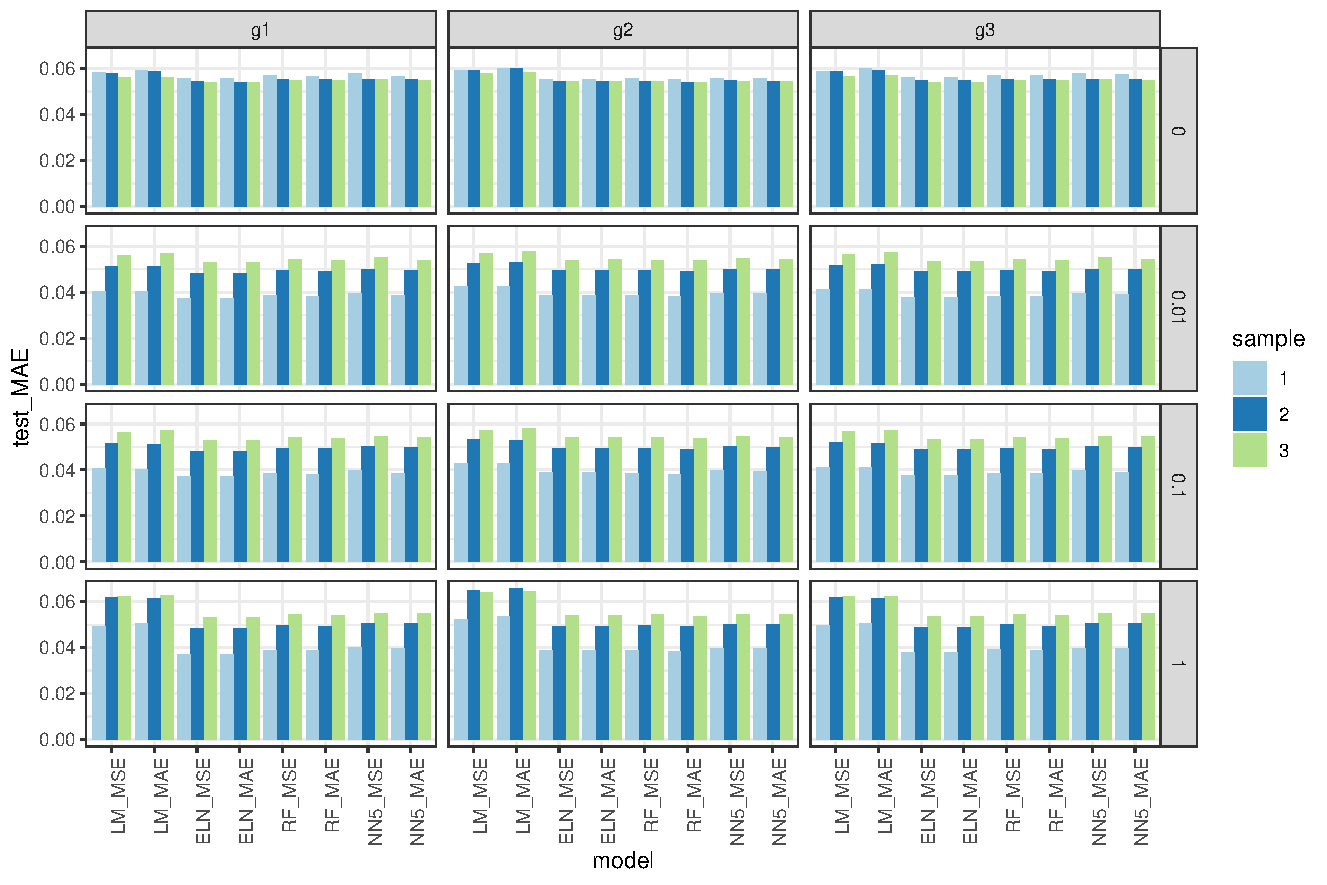
\includegraphics[max size = {\textwidth}{0.4\textheight}]{simulation_test_mae_pre_all.pdf}
		\caption{Simulation Test MAE}
		\floatfoot{Note: faceted by the different data generating processes at the top, and the degree of cross sectional correlation on the right. The y axis represents the MAE on the test set, and the x axis denotes the model (LM = Linear Model, ELN = Elastic Net, RF = Random Forest, NNX = Neural Network with X hidden layers), as well as the loss function it was fitted with respect to. The better performing loss function is bolded for emphasis. Note that only Neural Network 5, the of the neural networks, was shown here.}
		\label{fig:simulation_loss_metrics}
	\end{center}
\end{figure}

\begin{figure}[!htb]
	\begin{center}
		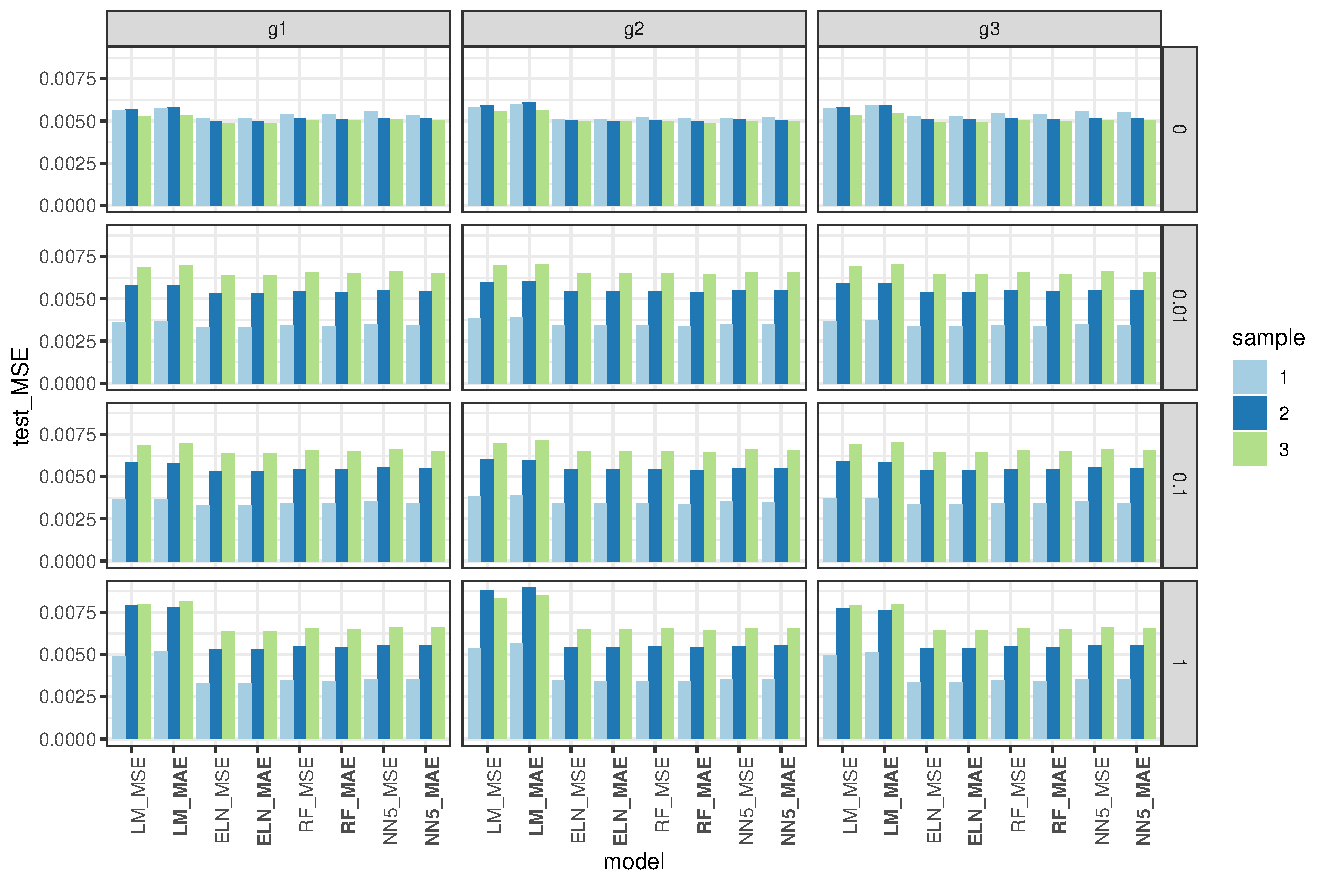
\includegraphics[max size = {\textwidth}{0.4\textheight}]{simulation_test_mse_pre_all.pdf}
	\end{center}
	\caption{Simulation Test MSE, see Figure \ref{fig:simulation_loss_metrics} for naming conventions}
\end{figure}

\begin{figure}[!htb]
	\begin{center}
		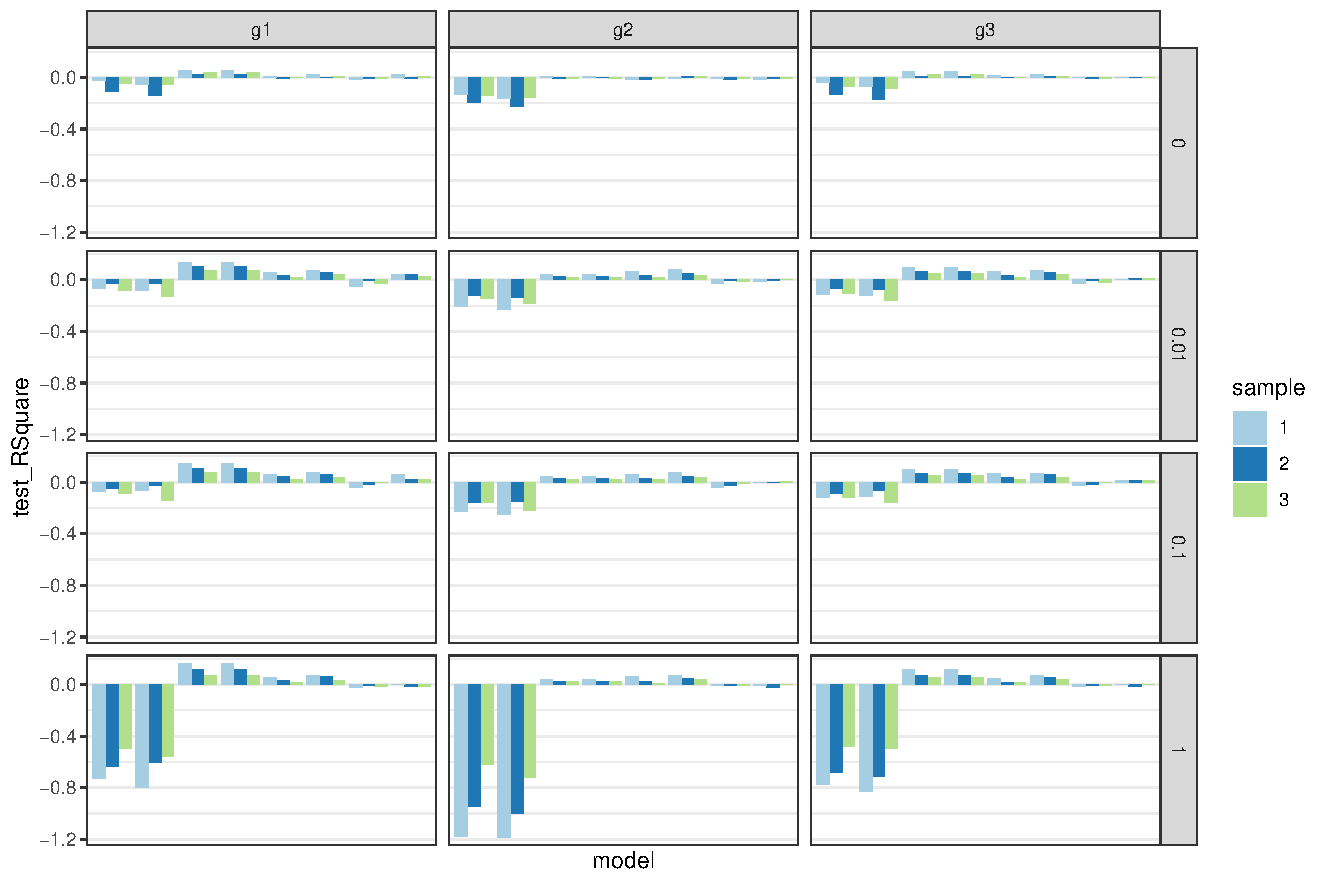
\includegraphics[max size = {\textwidth}{0.4\textheight}]{simulation_test_rsquare_pre_all.pdf}
	\end{center}
	\caption{Simulation Test MSE, see Figure \ref{fig:simulation_loss_metrics} for naming conventions}
\end{figure}

Across all specifications with a stochastic volatility component, we observe a decrease in prediction performance as the sample size increased according to the expanding window approach implemented. This is likely due a larger sample having a higher chance to experiences external shocks due to the stochastic volatility process, and thus a higher chance to experience large outliers in the training sample, leading to worse prediction performance. This indicates that machine learning performs poorly when the training data supplied contains more large outliers, and is still sensitive to such outliers even with the use of regularization and robust loss functions.

Focusing on the neural networks, we clearly see that they do not outperform any of the other machine learning models, even when the underlying data generating process is non-linear. This directly contradicts the result which \cite{gu_empirical_2018} find, even when considering the design with no cross sectional correlation and stochastic volatility (top row in graphs), which corresponds to their exact specification but with a multivariate macroeconomic series. We also find consistent evidence that deeper architectures provide better prediction performance, another result which contradicts \cite{gu_empirical_2018}'s conclusions that shallow learning may be better.

%% Causal Performance

Focusing on the factor selection capabilities of different models by looking at variable importance metrics however reveals a more interesting comparison between models. We can clearly observe that the elastic net outperforms all other models consistently in terms of assigning the correct relative importance to the true underlying regressors \footnote{($c_1.\text{constant}$, $c_2.\text{constant}$ and $c_3.x_3$ for $g1$ and $g_2$ specifications, and $c_1.\text{constant}$, $c_2.\text{constant}$ and $c_3.\text{constant}$ for $g_3$)}, even in settings with very high cross sectional correlation. 

In terms of finding the correct underlying regressors, we find that the penalized linear models perform the best at identifying the true data generating regressors, and that this appears to be mostly robust regardless of the amount of cross sectional correlation in the factor set. The penalized linear models are not perfect and their ability to correctly identify underlying regressors worsens as the data generating process becomes more non-linear. On these more difficult specifications, the penalized linear models are generally very conservative, sometimes only identifying a single covariate as important. This is most apparent on the $g_2$ specification. Occasionally, the elastic nets identified the incorrect covariates completely, though the relative importance assigned to them was small. 

The random forests and to a lesser extent the neural networks also correctly identified the correct underlying regressors, but struggled with adequately discerning relative importance among correlated regressors. This was became more apparent as the degree of cross sectional correlation increased (see decreasing relative importance of true underlying regressors in Figures \ref{fig:rf_sim_vi} and \ref{fig:nn_sim_vi} in Appendix). In the case of the random forests, this is to be expected, likely due to how the random forest algorithms work. The random forest algorithm is an ensemble of tree models, with each tree model only having access to a subset of all available predictors. If this subset does not include the true data generating predictor, then that particular tree will likely select the predictors which have the highest correlation with the true data generating predictor instead. Thus, the resulting ensemble model is likely to believe that cross sectionally correlated predictors are important, relative to the true underlying regressor. Due to the complexity of the neural networks, there does not exist a similar intuitive explanation for their factor selection ability.

\begin{landscape}
	\begin{figure}[!htb]
		\begin{center}
			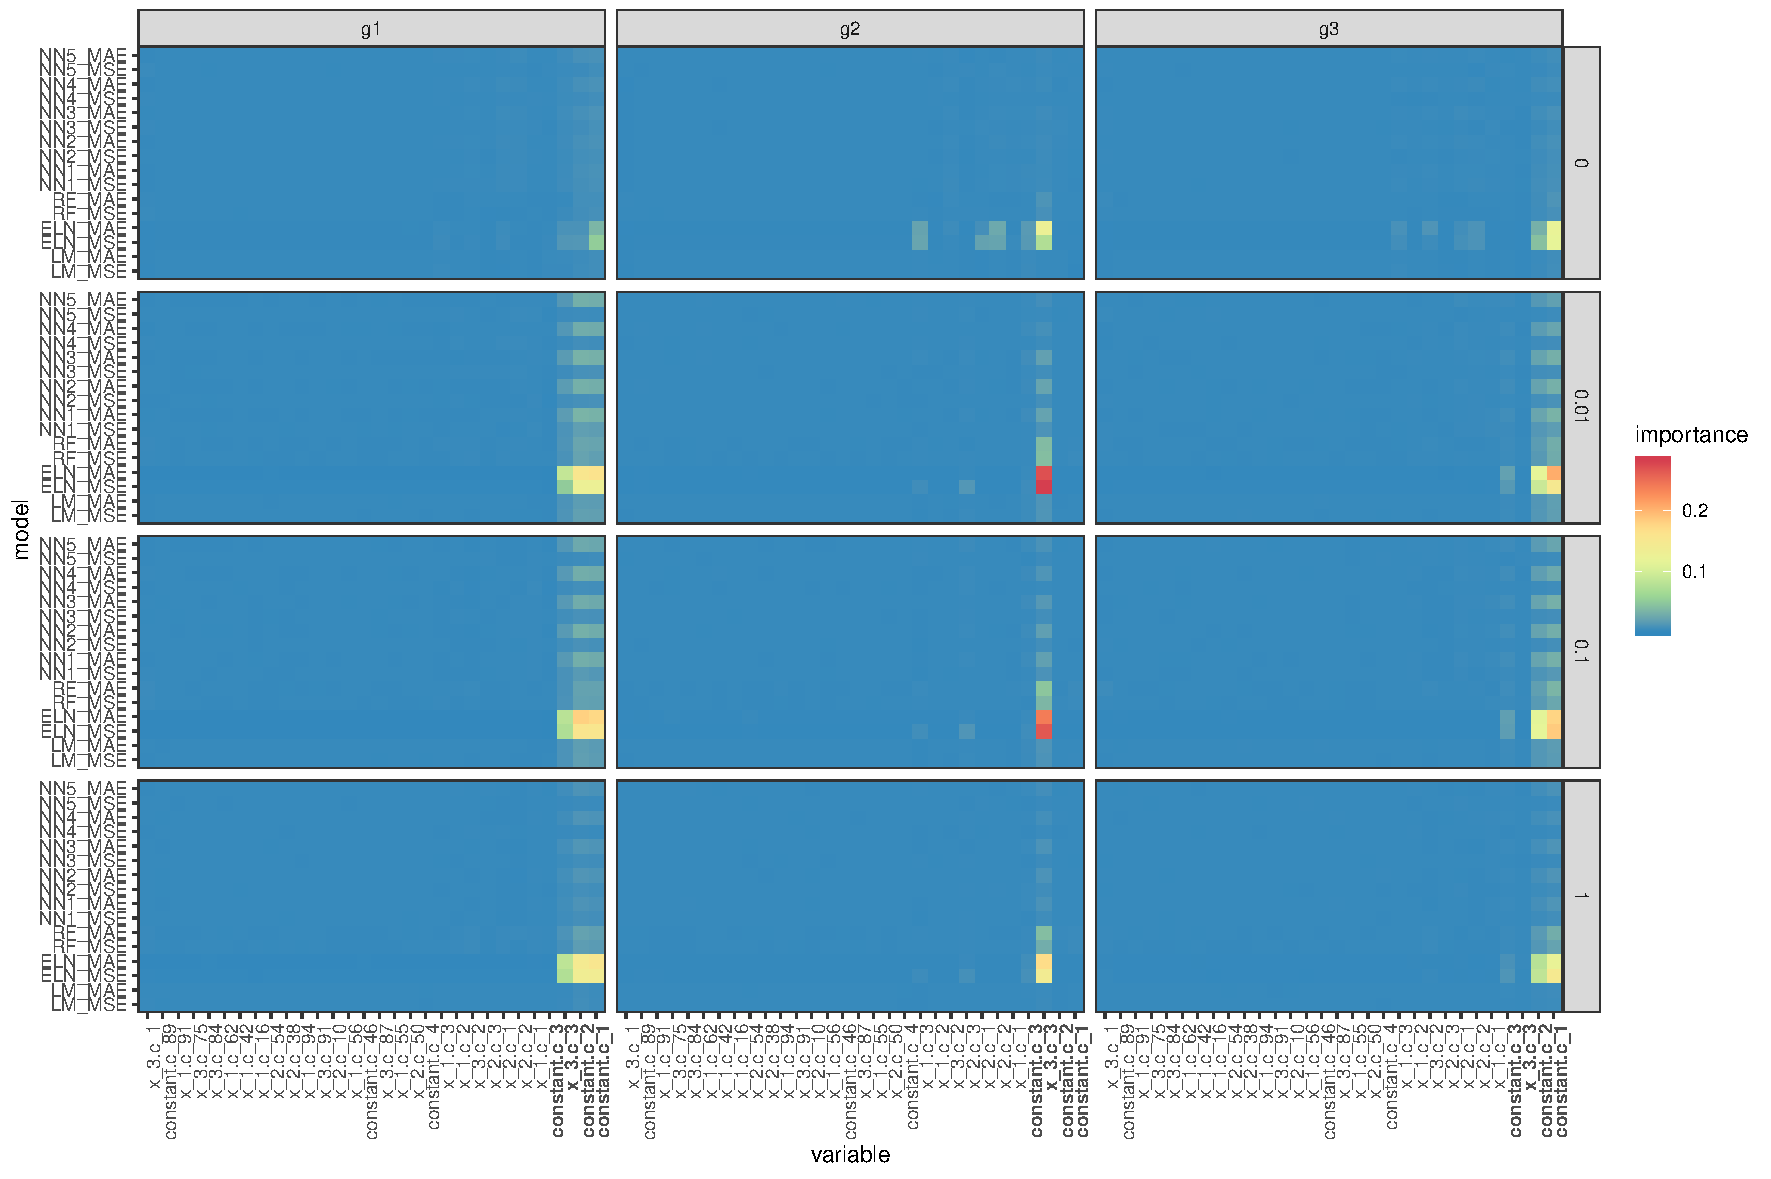
\includegraphics[max size = {23cm}{23cm}]{simulation_ave_vi_plot.pdf}
			\caption{Simulation Variable Importance averaged across all test samples}
			\floatfoot{Note: faceted by data generating specification at the top, and degree of cross-sectional correlation on the right. Model is on the y axis and follows the naming convention in Figure \ref{fig:simulation_loss_metrics}. Factor is on the x axis, and only contains the top 30 important factors, as measured by average importance across all samples and models. Note that the four true underlying factors are bolded.}
		\end{center}
	\end{figure}
\end{landscape}

The linear models, unsurprisingly, struggled with factor significance analysis with respect to both increasing cross sectional correlation and increasing non-linearities. This highlights the non-robustness and ineffectiveness of using traditional linear regression as documented by the literature; linear models were consistently observed to identify irrelevant regressors as important, especially as the degree of cross sectional correlation increased. Considering that the graphs represent the averaged variable importance metrics over different simulation realisations which each have random patterns of cross sectional correlation, this means that on a single simulation realization, the performance of linear models is significantly worse.

%% Brief other notes that are not too important

Of particular note are the instability of the machine learning models' hyperparameters across different training samples. For the elastic nets, the optimal value for $\alpha$ is generally 1 (corresponding to LASSO and thus a sparse representation), but it was not uncommon to observe $\alpha$ values swinging between values close to 0 (corresponding to ridge regression, and thus a dense representation) to 1 as the training sample moved forwards in time. As the penalized linear models consistently performed the best and still remained able to correctly identify the true covariates this is not a large issue, but it should be noted that this can lead to interpretation issues. For the random forests, it was similarly observed that the optimal value for $mtry$ (the number of variables subsetted) and $nodesize$ was highly non-robust. Again, given that the final prediction performance was consistent this is not a large issue, but can lead to some interpretation issues.

%%%%%%%%%%%%%%%%%%%%%%%%%%%%%%%%%%%%%%%%%%%%%%%%%%%%%%%%%%%%%%%%%%%%%%%%%%%%%%%%%%%%%%%%%%%%%%%%%%%

\newpage

\section{Empirical Study}

We conduct an empirical study as a final way to corroborate the findings of the properties of machine learning models which we observed in the simulation study. Though our simulation study was aimed at capturing the main features of observed data, the underlying data generating process for empirical returns is unknown. This study thus acts as a robustness check as to how machine learning performs on real world data, which can be significantly more complex and noisy than simulated contexts. Our two studies together can be thought of a repeated sampling exercise in exploring how machine learning methods perform on datasets which feature the ``stylized facts" of empirical returns. This empirical study also acts as a final validation against what has been reported in the literature.

Importantly, we find that our findings from the simulation study are largely corroborated for empirical returns data.

\subsection{Data}

We begin by considering monthly total individual equity returns from CRSP for all firms listed in the NYSE, AMEX and NASDAQ, starting from 1957 (starting date of the S\&P 500) and ending in December 2016, totalling 60 years. To build individual factors, we construct a factor set based on the cross section of returns literature. This data was sourced from and is the same data used in \cite{gu_empirical_2018}. Like our initial returns sample, it begins in March 1957 and ends in December 2016, totalling 60 years. It contains 94 stock level characteristics: 61 updated annually, 13 updated quarterly and 20 updated monthly, in addition to 74 industry dummies corresponding the the first two digits of the Standard Industrial Classification (SIC) codes. It is noted that this dataset so far contains all securities traded, including those with a CRSP share code other than 10 or 11 and thus includes instruments such as REITs and mutual funds, and those with a share price of less than \$5.

% Begin Cleaning

We detail our cleaning procedure of this dataset. To reduce the size of the dataset and increase feasibility, the dataset was filtered such that only stocks traded primarily on NASDAQ were included (using the PRIMEXCH variable from WRDS). Then, penny stocks (also referred to as microcaps in the literature) with a stock price of less than \$5 were filtered out, as is commonly done in the literature to reduce variability. Stocks without a share code of 10 or 11 (referring to equities) were filtered out, so that securities that are not equities were not included (such as REITs and trust funds). The dataset is provided in a monthly format, which means that many of the factors which are updated only quarterly or annually have very low levels of variability, which can lead to misleading results in the model fitting process. To achieve a balance between having a dataset with enough data points and variability among factors, the dataset was converted to a quarterly format. Quarterly returns were then constructed using the PRC variable according to actual returns (ie not logged differences):

\begin{equation}
	RET_t = \frac{PRC_t - PRC_{t-1}}{PRC_{t-1}}
\end{equation}

We allow all stocks which have a quarterly return to enter the dataset, even if they disappear from the dataset for certain periods, as opposed to only keeping stocks which appear continuously throughout the entire period. This was primarily done to reduce survivorship bias in the dataset, which can be very prevalent in financial data, and also allows for stocks which were unlisted and relisted again to feature in the dataset. This has the obvious drawback of introducing some bias in the dataset, as attrition in the dataset is likely to be non-random and correlated with the stocks' returns. 

The sic2 variable, corresponding to the stocks' Standard Industrial Classification (SIC) codes was also dropped. The SIC code system suffers from inconsistent logic in classifying companies, and as a system built for pre-1970s traditional industries has been slow in recognizing new and emerging industries. Indeed, WRDS explicitly cautions the use of SIC codes beyond the use of rough grouping of industries, warning that SIC codes are not strictly enforced by government agencies for accuracy, in addition to most large companies belonging to multiple SIC codes over time. Because of this latter point in particular, there can be inconsistencies on the correct SIC code for the same company depending on the data source. Dropping the sic2 variable also reduced the dimensionality of the dataset by 74 columns, significant increasing computational feasibility.

There existed a significant amount of missing data in the dataset. The dataset's columns were first examined, and any characteristics that had over 20\% of their data were removed. However, as the amount of missing data increases dramatically going further back in time, a balance between using more periods at the cost of removing more characteristics versus using less periods but keeping more characteristics was needed. 1993 Q3 was determined to be a reasonable time frame to begin the dataset, as there was a noticeable increase in data availability and quality after this time.  Missing characteristics were then imputed using their cross sectional medians for each year. 

We then follow \cite{gu_empirical_2018} and construct eight macroeconomic factors following the variable definitions in \cite{welch_comprehensive_2008}: dividend-price ratio (dp), earnings-price ratio (ep), book-to-market ratio (bm), net equity expansion (ntis), Treasury-bill rate (tbl), term spread (tms), default spread (dfy) and stock variance (svar). These factors were lagged by one period so as to be used to predict one period ahead quarterly returns. The treasury bill rate was also used from this source to proxy for the risk free rate in order to construct excess quarterly returns. 

\begin{table}
	\caption{Macroeconomic Factors, (\cite{welch_comprehensive_2008})}
	\label{macro_factors}
	\begin{center}
		\begin{tabular}{lccc} \hline
			No. & Acronym & Macroeconomic Factor \\ \hline
			1 & macro\_dp & Dividend Price Ratio \\
			2 & macro\_ep & Earnings Price Ratio \\
			3 & macro\_bm & Book to Market Ratio \\
			4 & macro\_ntis & Net Equity Expansion \\
			5 & macro\_tbl & Treasury Bill Rate \\
			6 & macro\_tms & Term Spread \\
			7 & macro\_dfy & Default Spread \\
			8 & macro\_svar & Stock Variance \\ \hline
		\end{tabular}
	\end{center}
\end{table}

The two sets of factors were then combined to form a baseline set of covariates, which we define throughout all methods and analysis as:

\begin{equation}
z_{i,t} = (1, x_t)' \otimes c_{i, t}
\end{equation}

where $c_{i,t}$ is a $P_c$ matrix of characteristics for each stock $i$, and $(1, x_t)'$ is a $P_x \times 1$ vector of macroeconomic predictors. $z_{i,t}$ is therefore a $P_x P_c$ vector of features for predicting individual stock returns and includes interactions between stock level characteristics and macroeconomic variables. The total number of covariates in this baseline set is $61 \times (8 + 1) = 549$\footnote{As the individual and macroeconomic factors can have similar names, individual and macroeconomic factors were prefixed with ind\_ and macro\_ respectively.}.
 
% Splitting Scheme
% Similar splitting scheme to simulation study used
% Training:Validation size ratio of 1.5, growing and moving forwards by 1 year
% To maintain feasibility, only 3 samples were conducted

The dataset was not normalized for all methods, as only penalized regression and neural networks are sensitive to normalization. For these two methods, the dataset was normalized such that each predictor column had 0 mean and 1 variance.

The final dataset spanned from 1993 Q3 to 2016 Q4 with 202, 066 individual observations.

We mimic the procedure used in the simulation study. For the sample splitting procedure, the dataset was split such that the training and validation sets were split such that the training set was approximately 1.5 times the length of the validation set, in order to predict a test set that is one year in length.

\begin{figure}[!htb]
	\begin{center}
		\begin{tabular}{|c|p{0.55cm}p{0.55cm}p{0.50cm}p{0.50cm}p{0.50cm}p{0.50cm}p{0.50cm}p{0.50cm}p{0.50cm}p{0.50cm}p{0.50cm}p{0.50cm}p{0.50cm}p{0.50cm}p{0.50cm}p{0.50cm}|}
			\hline
			Set No. &&&&&&&&&&&&&&&& \\
			\hline
			%%%%%%%%
			3 & \cellcolor{cyan} & \cellcolor{cyan} & \cellcolor{cyan} & \cellcolor{cyan} & \cellcolor{cyan} & \cellcolor{cyan} & \cellcolor{cyan} & \cellcolor{cyan} &
			\cellcolor{pink} & \cellcolor{pink} & \cellcolor{pink} & \cellcolor{pink} & \cellcolor{pink} & \cellcolor{pink} & \cellcolor{pink} & \cellcolor{olive} \\
			%%%%%%%%
			2 & \cellcolor{cyan} & \cellcolor{cyan} & \cellcolor{cyan} & \cellcolor{cyan} & \cellcolor{cyan} & \cellcolor{cyan} & \cellcolor{cyan} &
			\cellcolor{pink} & \cellcolor{pink} & \cellcolor{pink} & \cellcolor{pink} & \cellcolor{pink} & \cellcolor{pink} & \cellcolor{pink} & 	
			\cellcolor{olive} & NA \\
			%%%%%%%%
			1 & \cellcolor{cyan} & \cellcolor{cyan} & \cellcolor{cyan} & \cellcolor{cyan} & \cellcolor{cyan} & \cellcolor{cyan} &
			\cellcolor{pink} & \cellcolor{pink} & \cellcolor{pink} & \cellcolor{pink} & \cellcolor{pink} & \cellcolor{pink} & \cellcolor{pink} & \cellcolor{olive} & NA & NA \\
			\hline
			Time & 93Q3 & 93Q4 & 94 & 95 & 96 & ... & 06 & 07 & 08 & ... & 11 & 12 & 13 & 14 & 15 & 16 \\
			\hline
		\end{tabular}
		\medskip
		\begin{tabular}{|c|p{0.60cm}|}
			\hline
			Training & \cellcolor{cyan} \\
			\hline
			Validation & \cellcolor{pink} \\
			\hline
			Test & \cellcolor{olive} \\
			\hline
		\end{tabular}
	\end{center}
	\caption{Empirical Data Sample Splitting Procedure}
	\label{emp_sample_split_diag}
\end{figure}

\subsection{Empirical Data Results}

% Overall Results

In general, the empirical results are in remarkable agreement with the those obtained in the simulation study. In particular, we similarly see that the penalized linear models generally performing the best, with the random forest models offering slightly worse performance, occasionally outperforming penalized linear models. Machine learning models fitted with respect to median quantile loss were similarly observed to typically offer improvements across all machine learning models across all loss metrics. 

% Prediction Accuracy

In terms of prediction accuracy, we can see that in general the results of the simulation study were repeated: the elastic net models perform the best, followed by the random forests, then the neural networks, and finally the linear models. We note that the differences between each model using the MSE and MAE loss metrics are much more pronounced on empirical data. We similarly see that machine learning models perform better when fitted with respect to quantile loss instead of MSE. 

\begin{figure}[!htb]
	\begin{center}
		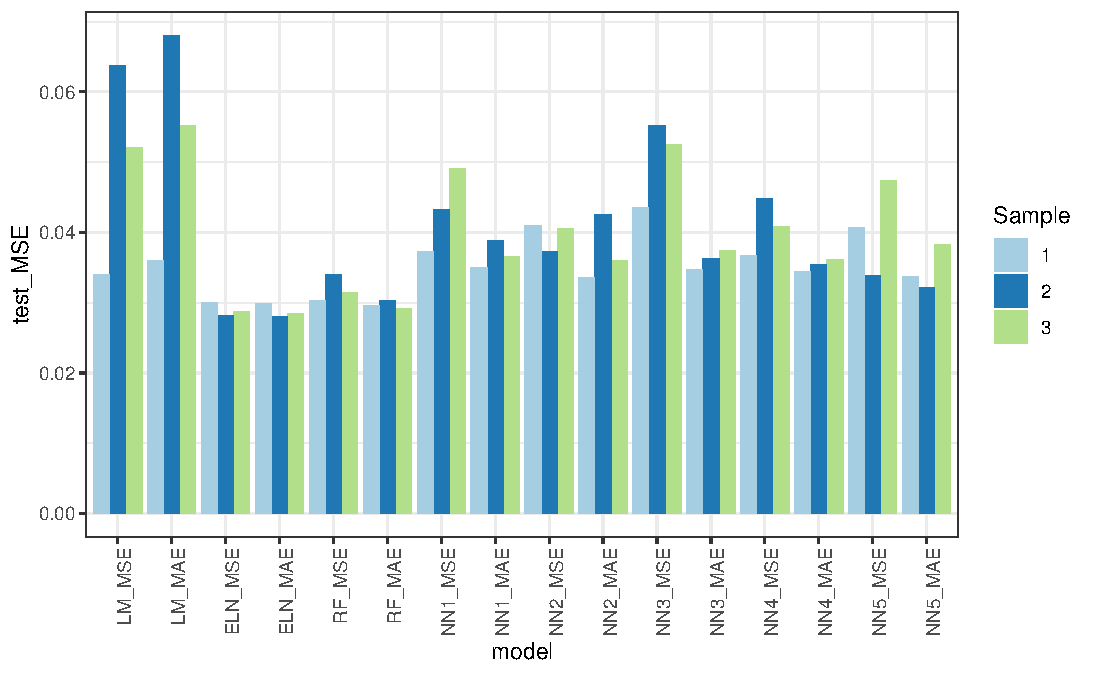
\includegraphics[max size = {\textwidth}{0.35\textheight}]{empirical_test_mse}
	\end{center}
	\caption{Empirical Test MSE}
	\floatfoot{Note: Test MSE on y axis, with model on x axis, following naming convention in Figure \ref{fig:simulation_loss_metrics}}
\end{figure}

Focusing on the neural networks specifically, their non-robustness is amplified on the empirical dataset, with some neural networks in some samples even performing worse than linear models. This was observed to be somewhat more common on neural networks fitted with respect to MSE, suggesting that they are indeed very sensitive to outliers in training data. We similarly observe some evidence that deeper neural networks perform better, though this result is less apparent to the lower robustness on empirical data.

Interestingly, we do not observe worsening performance as the training sample increases as we did in the simulation study. This suggests that the simulation design may have been too volatile when compared to the specific empirical time periods examined.

\begin{figure}[!htb]
	\begin{center}
		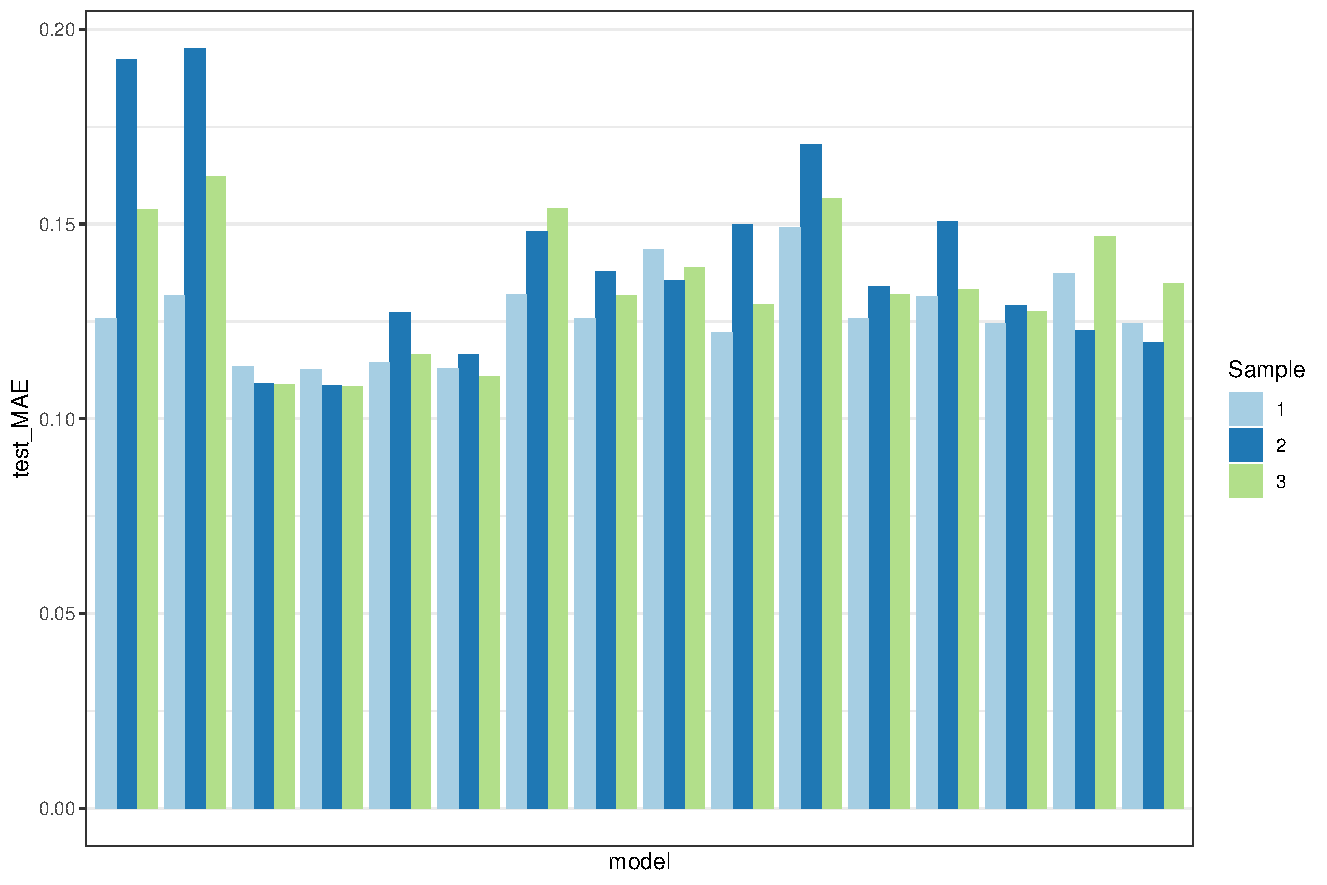
\includegraphics[max size = {\textwidth}{0.35\textheight}]{empirical_test_mae}
	\end{center}
	\caption{Empirical Test MAE}
	\floatfoot{Note: Test MAE on y axis, with model on x axis, following naming convention in Figure \ref{fig:simulation_loss_metrics}}
\end{figure}

\begin{figure}[!htb]
	\begin{center}
		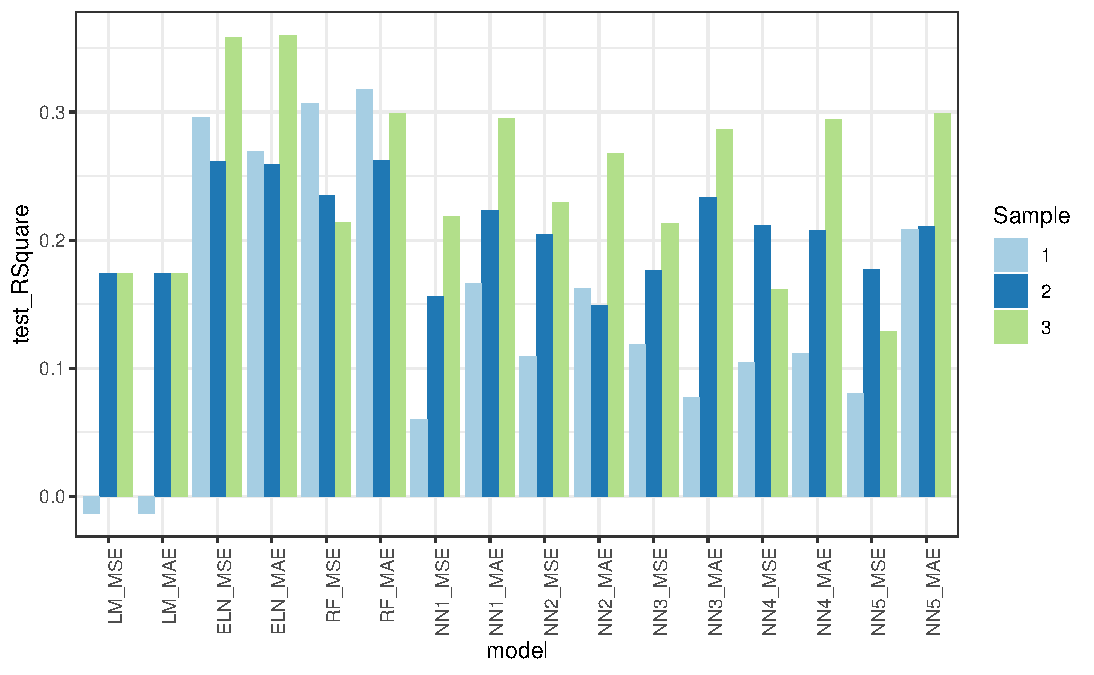
\includegraphics[max size = {\textwidth}{0.35\textheight}]{empirical_test_rsquare}
	\end{center}
	\caption{Empirical Test Predictive R-Squared}
	\floatfoot{Note: Test Predictive R-Squared on y axis, with model on x axis, following naming convention in Figure \ref{fig:simulation_loss_metrics}}
\end{figure}

%% Causal Inference

As the data generating process for empirical returns is unknown, the variable importance results cannot be directly compared with those of the simulation study. Even so, we see similar results: the elastic net and random forest models tend to agree on the same subset of predictors, but the random forest struggles to discern between highly correlated regressors. Similar to the prediction performance results, neural networks perform poorly.

\begin{figure}[!htb]
	\begin{center}
		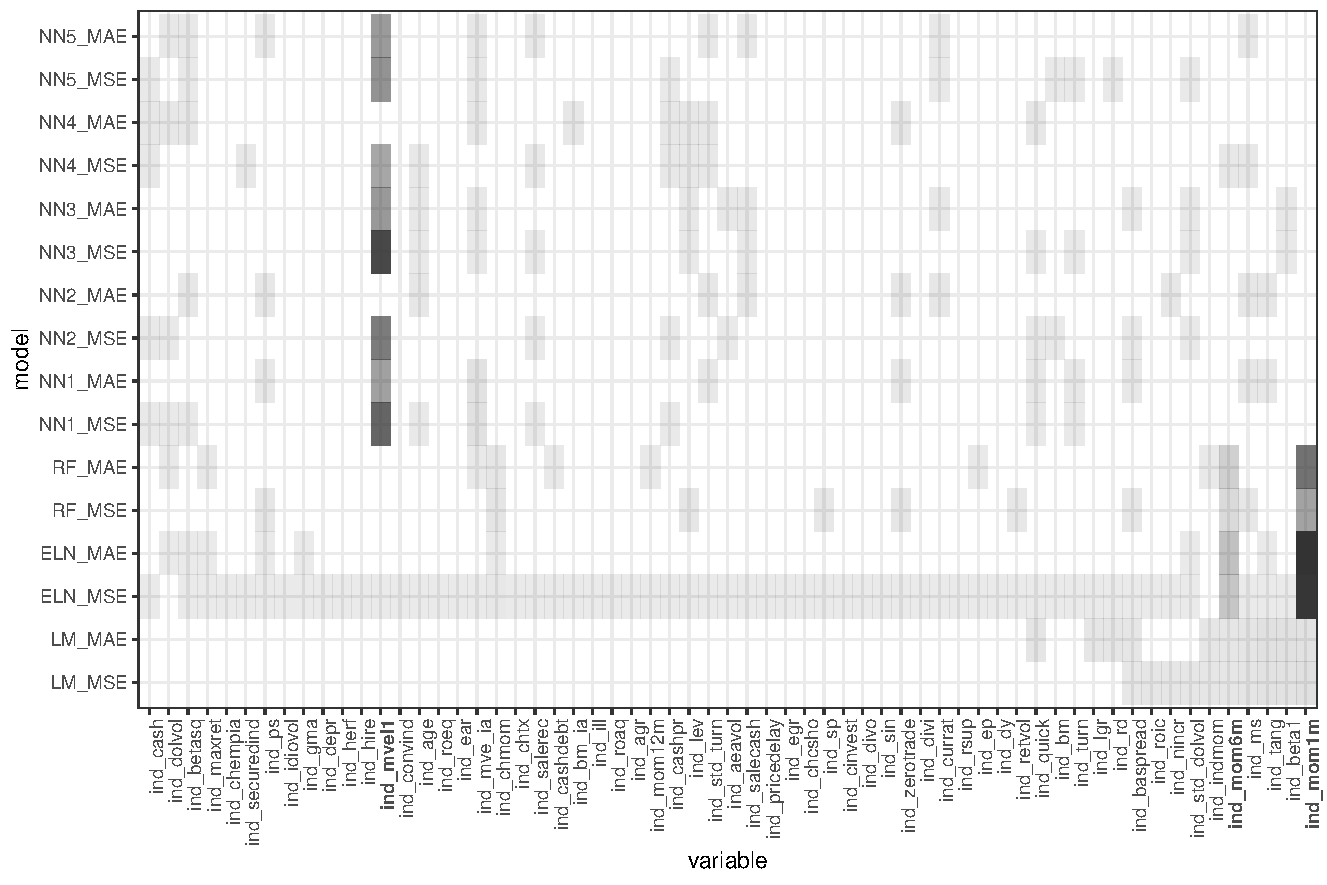
\includegraphics[max size = {\textwidth}{0.35\textheight}]{empirical_sample_all_vi_ind}
		\caption{Empirical Individual Factor Importance, averaged across all training samples}
		\floatfoot{Individual factors shown on x axis, with most important variables bolded (see Table \ref{ind_factors} in Appendix for definitions)}
	\end{center}
\end{figure}

\begin{figure}[!htb]
	\label{empirical_macro_facet}
	\begin{center}
		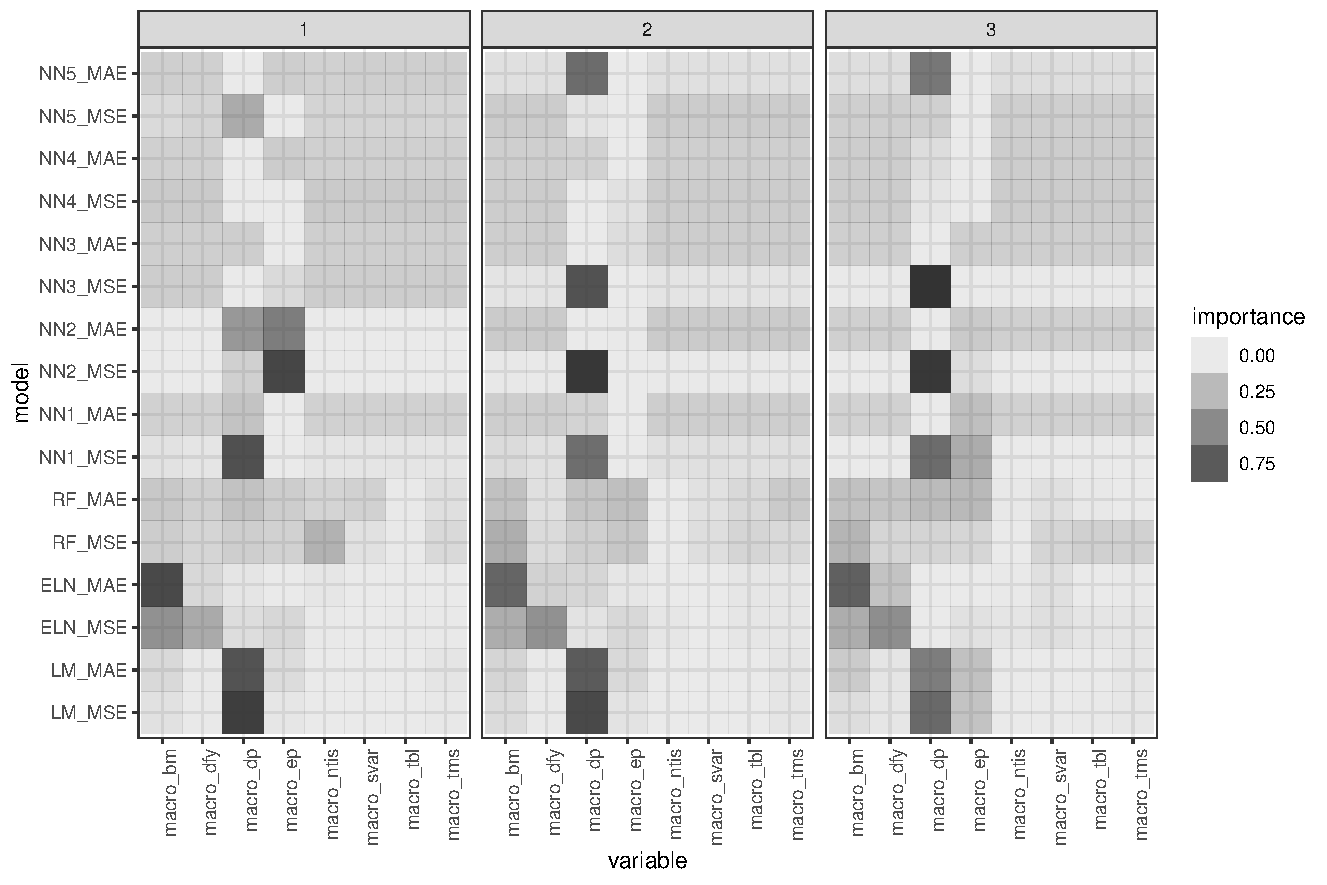
\includegraphics[max size = {\textwidth}{0.35\textheight}]{empirical_sample_all_vi_macro_facet}
		\caption{Empirical Macroeconomic Factor Importance, faceted by training sample}
		\floatfoot{Macroeconomic Factors shown on x axis (see Table \ref{macro_factors} for definitions)}
	\end{center}
\end{figure}

If we focus on the two top performing models of elastic net and random forest, we see that they consistently pick out the 1 month and 6 month momentum factors out of the individual characteristics as important, and the book-to-market and default yield spread factors out of the macroeconomic factors are important. In general though, the variable importance metrics are less consistent for the random forests, and it should be noted in particular that the random forest tends to determine factors highly correlated with momentum as important, such as change in moment, dollar trading volume and return volatility. Looking at the macroeconomic factors, penalized linear models tend to identify the average book to market ratio and the default spread as the most important macroeconomic factors. On the macroeconomic factor set, the random forests were inconsistent with the elastic nets, and tended to assign very similar variable importance metrics to most macroeconomic factors.

The neural networks tended to believe that the market value factor was the most important among the individual factors, a result not repeated by any of the other models considered. Within the macroeconomic factors, the neural networks identified and the dividend-price ratio and earnings-price ratio as the most important among the macroeconomic factors, though these results were highly non-robust across different architectures, loss functions and training samples.

Interestingly, we find that the linear models assign the controversial dividend price ratio macroeconomic factor as highly important, a result mirrored only with the neural networks Their variable importance for individual factors across different training samples is highly non-robust, with the important variables almost completely changing year to year. The linear models consistently identified the controversial dividend-price ratio as important, a result that was somewhat consistent with the neural networks. 

The overall results again contradict the results of \cite{gu_empirical_2018}, who conclude that all of the machine methods agree on the same subset of important factors. Indeed, we only see consistency in variable importance between the elastic nets and random forests on the individual factors only - all other variable importance metrics were either inconsistent between different models, or non-robust.

%% Other Notes

All models considered typically preferred sparse parameterizations. That is, most if not all of the individual factors had little to no importance across all models.\footnote{Note that because the variable importance here was not evaluated explicitly for each pairwise interaction term, some of the individual factors appear as slightly important. This is because setting an individual factor to zero also sets some of the macroeconomic pairwise terms to zero, increasing its apparent importance.}

\newpage

\section{Conclusion}

Our findings demonstrate that the field of machine learning may offer certain tools to improve stock prediction and identification of true underlying factors. Penalized linear models and to a lesser extent, random forests are the best performing methods in the analysis undertaken.

Importantly, we find that the feed-forward neural network architectures considered by \cite{gu_empirical_2018} fail in the context of stock return prediction, at both prediction performance and variable importance analysis. This result is consistent across a variety of simulated datasets, as well as empirical data. We also find weak evidence that deeper neural networks with more hidden layers perform better, though this result, like the performance of neural networks in general, is non-robust.

Lastly, we find that the top performing models - the penalized linear models and random forests, tend to agree and correctly identify the correct underlying regressors in simulated contexts, as well as agree on the same subset of factors which are important in empirical contexts. We find that of all the most considered, the penalized linear models are the most consistent at identifying true underlying regressors through the simulation study. We find that in the empirical setting, among the individual factors the individual 1 and 6 month momentum factors are the most powerful predictors of stock returns, according to the penalized linear models and random forests. 

Across all models except for linear models, we find that minimizing quantile loss yields better prediction performance.

The overall findings of this paper differ from the sparse literature on machine learning methods in empirical finance. However, the performance of the penalized linear models with respect to both out of sample prediction performance and variable importance analysis is promising, and our findings show that machine learning provides some tools which may aid in the problems of stock return prediction and risk factor selection in the financial world. 

\newpage

\section{Appendix}

\subsection{Data}

%% Macroeconomic Factor Table

\begin{table}[!htb]
	\caption{Macroeconomic Factors}
	\begin{center}
		\begin{tabular}{lccc} \hline
			No. & Acronym & Macroeconomic Factor \\ \hline
			1 & macro\_dp & Dividend Price Ratio \\
			2 & macro\_ep & Earnings Price Ratio \\
			3 & macro\_bm & Book to Market Ratio \\
			4 & macro\_ntis & Net Equity Expansion \\
			5 & macro\_tbl & Treasury Bill Rate \\
			6 & macro\_tms & Term Spread \\
			7 & macro\_dfy & Default Spread \\
			8 & macro\_svar & Stock Variance \\ \hline
		\end{tabular}
	\end{center}
\end{table}

%% Individual Factor Table

\begin{landscape}
	\footnotetext{The factor was included in the original dataset provided by \cite{gu_empirical_2018}, but was not used due to missing data issues}
	\begin{center}
		\label{ind_factors}
		\begin{longtable}{lllllll}
			\caption{Individual Factors} \\ \hline
			No. & Acronym & Firm Characteristic & Author(s) & Data Source & Frequency \\ \hline
			1 & ind\_absacc\footnotemark[\value{footnote}] & Absolute Accruals & 
				\cite{bandyopadhyay_accrual_2010} & Compustat & Annual \\
			2 & ind\_acc\footnotemark[\value{footnote}] & Working capital accruals & 
				\cite{sloan_stock_1996} & Compustat & Annual \\
			3 & ind\_aeavol & Abnormal earnings announcement volume & 
				\cite{lerman_high-volume_2008} & Compustat & Quarterly \\
			4 & ind\_age & \# years since first Compustat coverage & 
				\cite{jiang_information_2005} & Compustat & Annual \\
			5 & ind\_agr & Asset growth & 
				\cite{cooper_asset_2008} & Compustat & Annual \\
			6 & ind\_baspread & Bid-ask spread & 
				\cite{amihud_effects_1989} & Compustat & Monthly \\
			7 & ind\_beta & Beta & 
				\cite{fama_risk_1973} & Compustat & Monthly \\
			8 & ind\_betasq & Beta squared & 
				\cite{fama_risk_1973} & Compustat & Monthly \\
			9 & ind\_bm & Book-to-market & 
				\cite{rosenberg_persuasive_1985} & Compustat & Annual \\
			10 & ind\_bm\_ia & Industry-adjusted book to market & 
				\cite{asness_predicting_2000} & Compustat & Quarterly \\
			%%%%%%%%%%%%%%%%%%%%%%%%%%%%%%%%%%%%%%%%%%%%%%%%%%%%%%%%%%%%%%%%%%%%%%%%%%%%%%%
			11 & ind\_cash & Cash holdings & 
				\cite{palazzo_cash_2012} & Compustat & Annual \\
			12 & ind\_cashdebt & Cashflow to debt & 
				\cite{ou_financial_1989} & Compustat & Annual \\
			13 & ind\_cashpr & Cash productivity & 
				\cite{chandrashekar_productivity_2009} & Compustat & Annual \\
			14 & ind\_cfp\footnotemark[\value{footnote}] & Cashflow to price ratio & 
				\cite{desai_value-glamour_2004} & Compustat & Annual \\
			15 & ind\_cfp\_ia\footnotemark[\value{footnote}] & Industry-adjusted cashfow to price ratio & 
				\cite{asness_predicting_2000} & Compustat & Annual \\
			16 & ind\_chatoia\footnotemark[\value{footnote}] & Industry-adjusted change in asset turnover & 
				\cite{soliman_use_2008} & Compustat & Annual \\
			17 & ind\_chcsho & Change in shares outstanding & 
				\cite{pontiff_share_2008} & Compustat & Annual \\
			18 & ind\_chempia & Industry-adjusted change in employee & 
				\cite{asness_predicting_2000} & Compustat & Annual \\
			19 & ind\_chinv\footnotemark[\value{footnote}] & Change in inventory & 
				\cite{thomas_inventory_2002} & Compustat & Annual \\
			%%%%%%%%%%%%%%%%%%%%%%%%%%%%%%%%%%%%%%%%%%%%%%%%%%%%%%%%%%%%%%%%%%%%%%%%%%%%%%%
			20 & ind\_chmom & Change in 6-month momentum & 
				\cite{gettleman_acceleration_2006} & Compustat & Monthly \\
			21 & ind\_chpmia\footnotemark[\value{footnote}] & Industry-adjusted change in profit margin & 
				\cite{soliman_use_2008} & Compustat & Annual \\
			22 & ind\_chtx & Change in tax expense & 
				\cite{thomas_tax_2011} & Compustat & Quarterly \\
			23 & ind\_cinvest & Corporate investment & 
				\cite{titman_capital_2004} & Compustat & Quarterly \\
			24 & ind\_convind & Convertible debt indicator & 
				\cite{valta_strategic_2016} & Compustat & Annual \\
			25 & ind\_currat & Current ratio & 
				\cite{ou_financial_1989} & Compustat & Annual \\
			26 & ind\_depr & Depreciation / PP\&E & 
				\cite{holthausen_prediction_1992} & Compustat & Annual \\
			27 & ind\_divi & Dividend initiation & 
				\cite{michaely_price_1995} & Compustat & Annual \\
			28 & ind\_divo & Dividend omission & 
				\cite{michaely_price_1995} & Compustat & Annual \\
			29 & ind\_dolvol & Dollar trading volume & 
				\cite{chordia_trading_2001} & Compustat & Monthly \\
			%%%%%%%%%%%%%%%%%%%%%%%%%%%%%%%%%%%%%%%%%%%%%%%%%%%%%%%%%%%%%%%%%%%%%%%%%%%%%%%
			30 & ind\_dy & Dividend to price & 
				\cite{litzenberger_effects_1982} & Compustat & Annual \\
			31 & ind\_ear & Earnings announcement return & 
				\cite{brandt_earnings_2008} & Compustat & Quarterly \\
			32 & ind\_egr & Growth in common shareholder eq & 
				\cite{richardson_accrual_2005} & Compustat & Annual \\
			33 & ind\_ep & Earnings to price & 
				\cite{basu_investment_1977} & Compustat & Annual \\
			34 & ind\_gma & Gross profitability & 
				\cite{novy-marx_other_2013} & Compustat & Annual \\
			35 & ind\_grCAPX\footnotemark[\value{footnote}] & Growth in capital expenditures & 
				\cite{anderson_empirical_2006} & Compustat & Annual \\
			36 & ind\_grltnoa\footnotemark[\value{footnote}] & Growth in long term net operating assets & 
				\cite{fairfield_accrued_2003} & Compustat & Annual \\
			37 & ind\_herf & Industry sales concentration & 
				\cite{hou_industry_2006} & Compustat & Annual \\
			38 & ind\_hire & Employee growth rate & 
				\cite{belo_labor_2014} & Compustat & Annual \\
			39 & ind\_idiovol & Idiosyncratic return volatility & 
				\cite{ali_arbitrage_2003} & Compustat & Monthly \\
			%%%%%%%%%%%%%%%%%%%%%%%%%%%%%%%%%%%%%%%%%%%%%%%%%%%%%%%%%%%%%%%%%%%%%%%%%%%%%%%
			40 & ind\_ill & Illiquidity & 
				\cite{amihud_illiquidity_2002} & Compustat & Monthly \\
			41 & ind\_indmom & Industry momentum & 
				\cite{moskowitz_industries_1999} & Compustat & Monthly \\
			42 & ind\_invest\footnotemark[\value{footnote}] & Capital expenditures and inventory & 
				\cite{chen_better_2010} & Compustat & Annual \\
			43 & ind\_lev & Leverage & 
				\cite{bhandari_debt/equity_1988} & Compustat & Annual \\
			44 & ind\_lgr & Growth in long-term debt & 
				\cite{richardson_accrual_2005} & Compustat & Annual \\
			45 & ind\_maxret & Maximum daily return & 
				\cite{bali_maxing_2011} & Compustat & Monthly \\
			46 & ind\_mom12m & 12-month momentum & 
				\cite{jegadeesh_evidence_1990} & Compustat & Monthly \\
			47 & ind\_mom1 & 1-month momentum & 
				\cite{jegadeesh_returns_1993} & Compustat & Monthly \\
			48 & ind\_mom36m\footnotemark[\value{footnote}] & 36-month momentum & 
				\cite{jegadeesh_returns_1993} & Compustat & Monthly \\
			49 & ind\_mom6m & 6-month momentum & 
				\cite{jegadeesh_returns_1993} & Compustat & Monthly \\
			%%%%%%%%%%%%%%%%%%%%%%%%%%%%%%%%%%%%%%%%%%%%%%%%%%%%%%%%%%%%%%%%%%%%%%%%%%%%%%%
			50 & ind\_ms & Financial statement score & 
				\cite{mohanram_separating_2005} & Compustat & Quarterly \\
			51 & ind\_mvel1 & Size & 
				\cite{banz_relationship_1981} & Compustat & Monthly \\
			52 & ind\_mve\_ia & Industry-adjusted size & 
				\cite{asness_predicting_2000} & Compustat & Annual \\
			53 & ind\_nincr & Number of earnings increases & 
				\cite{barth_market_1999} & Compustat & Quarterly \\
			54 & ind\_operprof\footnotemark[\value{footnote}] & Operating profitability & 
				\cite{fama_five-factor_2015} & Compustat & Annual \\
			55 & ind\_orgcap\footnotemark[\value{footnote}] & Organizational capital & 
				\cite{eisfeldt_organization_2013} & Compustat & Annual \\
			56 & ind\_pchcapx\_ia\footnotemark[\value{footnote}] & Industry adjusted \% change in capital expenditures & 
				\cite{abarbanell_abnormal_1998} & Compustat & Annual \\
			57 & ind\_pchcurrat\footnotemark[\value{footnote}] & \% change in current ratio & 
				\cite{ou_financial_1989} & Compustat & Annual \\
			58 & ind\_pchdepr\footnotemark[\value{footnote}] & \% change in depreciation & 
				\cite{holthausen_prediction_1992} & Compustat & Annual \\
			59 & ind\_pchgm\_pchsale\footnotemark[\value{footnote}] & \% change in gross margin - \% change in sales & 
				\cite{abarbanell_abnormal_1998} & Compustat & Annual \\
			%%%%%%%%%%%%%%%%%%%%%%%%%%%%%%%%%%%%%%%%%%%%%%%%%%%%%%%%%%%%%%%%%%%%%%%%%%%%%%%
			60 & ind\_pchquick\footnotemark[\value{footnote}] & \% change in quick ratio & 
				\cite{ou_financial_1989} & Compustat & Annual \\
			61 & ind\_pchsale\_pchinvt\footnotemark[\value{footnote}] & \% change in sales - \% change in inventory & 
				\cite{abarbanell_abnormal_1998} & Compustat & Annual \\
			62 & ind\_pchsale\_pchrect\footnotemark[\value{footnote}] & \% change in sales - \% change in A/R & 
				\cite{abarbanell_abnormal_1998} & Compustat & Annual \\
			63 & ind\_pchsale\_pchxsga\footnotemark[\value{footnote}] & \% change in sales - \% change in SG & 
				\cite{abarbanell_abnormal_1998} & Compustat & Annual \\
			64 & ind\_pchsaleinv\footnotemark[\value{footnote}] & \% change sales-to-inventory & 
				\cite{ou_financial_1989} & Compustat & Annual \\
			65 & ind\_pctacc\footnotemark[\value{footnote}] & Percent accruals & 
				\cite{hafzalla_percent_2011} & Compustat & Annual \\
			66 & ind\_pricedelay & Price delay & 
				\cite{hou_market_2005} & Compustat & Monthly \\
			67 & ind\_ps & Financial statements score & 
				\cite{piotroski_value_2000} & Compustat & Annual \\
			68 & ind\_quick & Quick ratio & 
				\cite{ou_financial_1989} & Compustat & Annual \\
			69 & ind\_rd & R\&D increase & 
				\cite{eberhart_examination_2004} & Compustat & Annual \\
			%%%%%%%%%%%%%%%%%%%%%%%%%%%%%%%%%%%%%%%%%%%%%%%%%%%%%%%%%%%%%%%%%%%%%%%%%%%%%%%
			70 & ind\_rd\_mve\footnotemark[\value{footnote}] & R\&D to market capitalization & 
				\cite{guo_explaining_2006} & Compustat & Annual \\
			71 & ind\_rd\_sale\footnotemark[\value{footnote}] & R\&D to sales & 
				\cite{guo_explaining_2006} & Compustat & Annual \\
			72 & ind\_realestate\footnotemark[\value{footnote}] & Real estate holdings & 
				\cite{tuzel_corporate_2010} & Compustat & Annual \\
			73 & ind\_retvol & Return volatility & 
				\cite{ang_cross-section_2006} & Compustat & Monthly \\
			74 & ind\_roaq & Return on assets & 
				\cite{balakrishnan_post_2010} & Compustat & Quarterly \\
			75 & ind\_roavol\footnotemark[\value{footnote}] & Earnings volatility & 
				\cite{francis_costs_2004} & Compustat & Quarterly \\
			76 & ind\_roeq & Return on equity & 
				\cite{hou_digesting_2015} & Compustat & Quarterly \\
			77 & ind\_roic & Return on invested capital & 
				\cite{brown_productivity_2007} & Compustat & Annual \\
			78 & ind\_rsup & Revenue surprise & 
				\cite{kama_market_2009} & Compustat & Quarterly \\
			79 & ind\_salecash & Sales to cash & 
				\cite{ou_financial_1989} & Compustat & Annual \\
			%%%%%%%%%%%%%%%%%%%%%%%%%%%%%%%%%%%%%%%%%%%%%%%%%%%%%%%%%%%%%%%%%%%%%%%%%%%%%%%
			80 & ind\_saleinv\footnotemark[\value{footnote}] & Sales to inventory & 
				\cite{ou_financial_1989} & Compustat & Annual \\
			81 & ind\_salerec & Sales to receivables & 
				\cite{ou_financial_1989} & Compustat & Annual \\
			82 & ind\_secured\footnotemark[\value{footnote}] & Secured debt & 
				\cite{valta_strategic_2016} & Compustat & Annual \\
			83 & ind\_securedind & Secured debt indicator & 
				\cite{valta_strategic_2016} & Compustat & Annual \\
			84 & ind\_sgr\footnotemark[\value{footnote}] & Sales growth & 
				\cite{barbee_jr_salesprice_1996} & Compustat & Annual \\
			85 & ind\_sin & Sin stocks & 
				\cite{hong_price_2009} & Compustat & Annual \\
			86 & ind\_sp & Sales to price & 
				\cite{barbee_jr_salesprice_1996} & Compustat & Annual \\
			87 & ind\_std\_dolvol & Volatility of liquidity (dollar trading volume) & 
				\cite{chordia_trading_2001} & Compustat & Annual \\
			88 & ind\_std\_turn & Volatility of liquidity (share turnover) & 
				\cite{chordia_trading_2001} & Compustat & Monthly \\
			89 & ind\_stdacc\footnotemark[\value{footnote}] & Accrual volatility & 
				\cite{bandyopadhyay_accrual_2010} & Compustat & Monthly \\
			%%%%%%%%%%%%%%%%%%%%%%%%%%%%%%%%%%%%%%%%%%%%%%%%%%%%%%%%%%%%%%%%%%%%%%%%%%%%%%%
			90 & ind\_stdcf\footnotemark[\value{footnote}] & Cashflow volatility & 
				\cite{huang_cross_2009} & Compustat & Quarterly \\
			91 & ind\_tang & Debt capacity/rm tangibility & 
				\cite{almeida_financial_2007} & Compustat & Quarterly \\
			92 & ind\_tb\footnotemark[\value{footnote}] & Tax income to book income & 
				\cite{lev_market-based_1982} & Compustat & Annual \\
			93 & ind\_turn & Share turnover & 
				\cite{datar_liquidity_1998} & Compustat & Monthly \\
			94 & ind\_zerotrade & Zero trading days & 
				\cite{liu_liquidity-augmented_2006} & Compustat & Monthly \\ \hline	
		\end{longtable}
	\end{center}
\end{landscape}

\newpage

\subsection{Additional Results}

\subsubsection{Simulation Study}

\begin{figure}[!htb]
	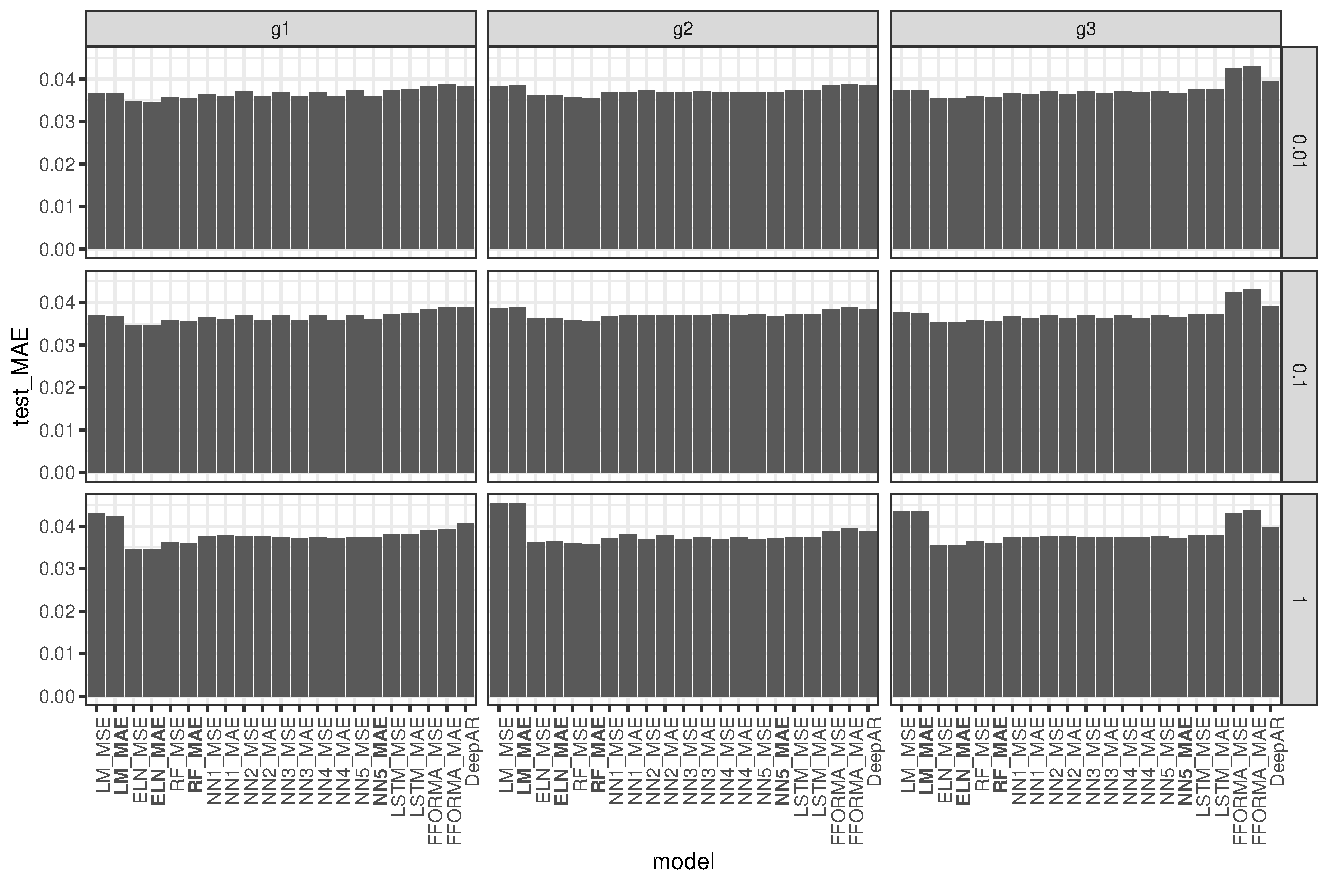
\includegraphics[max size = {\textwidth}{0.5\textheight}]{simulation_test_mae.pdf}
	\caption{Simulation Test MAE}
\end{figure}

\begin{figure}[!htb]
	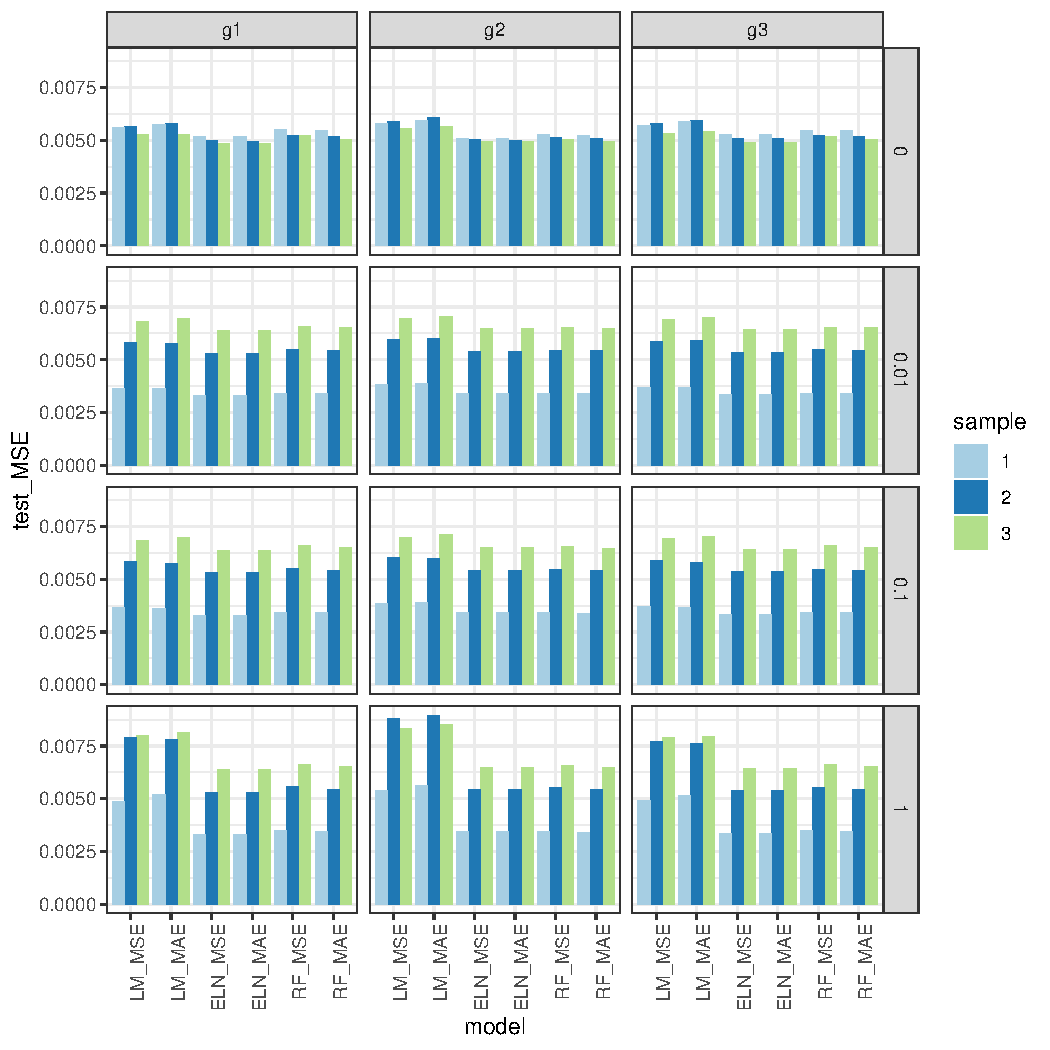
\includegraphics[max size = {\textwidth}{0.5\textheight}]{simulation_test_mse.pdf}
	\caption{Simulation Test MSE}
\end{figure}

\begin{figure}
	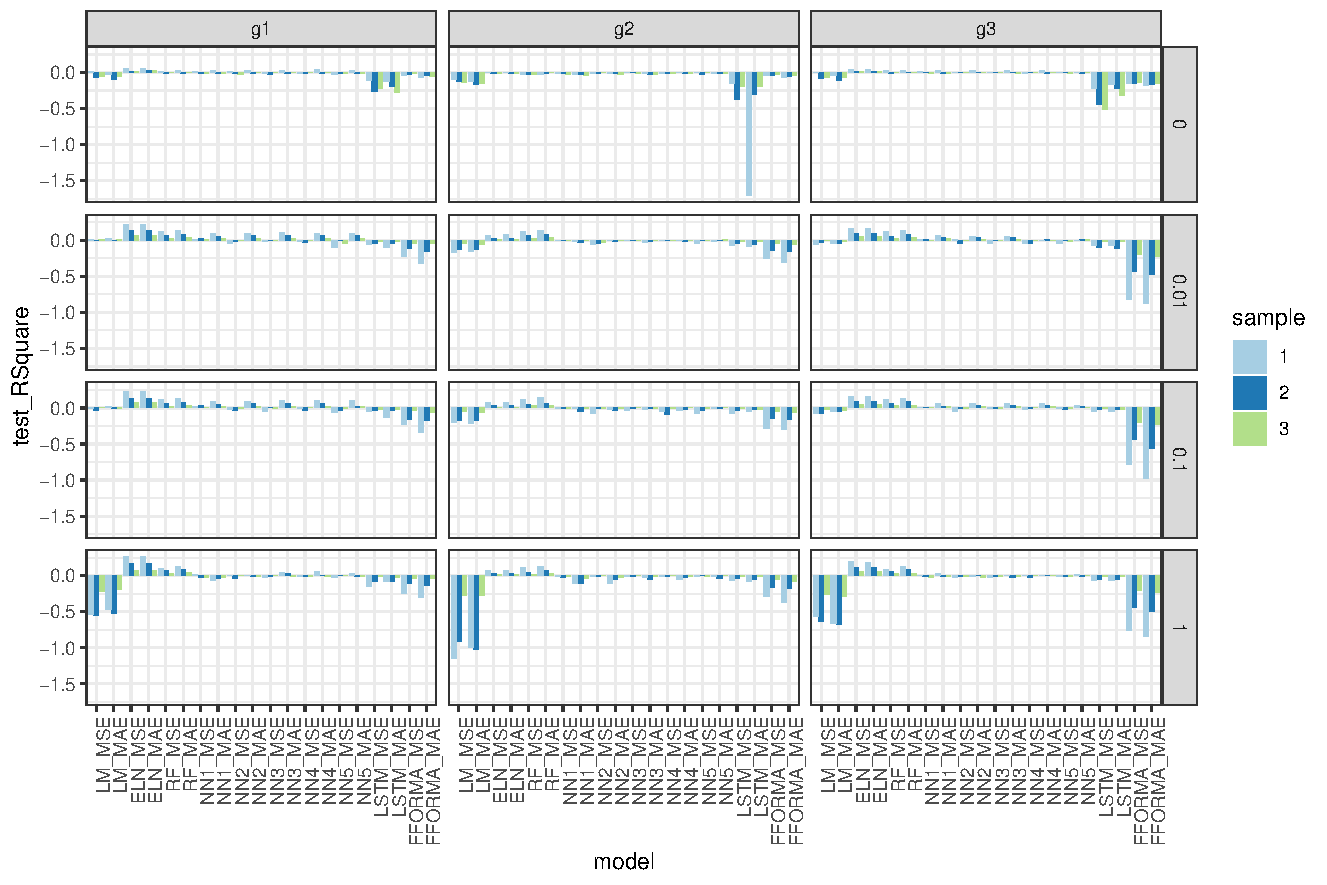
\includegraphics[max size = {\textwidth}{0.5\textheight}]{simulation_test_rsquare.pdf}
	\caption{Simulation Test R Squared}
\end{figure}

\begin{figure}[!htb]
	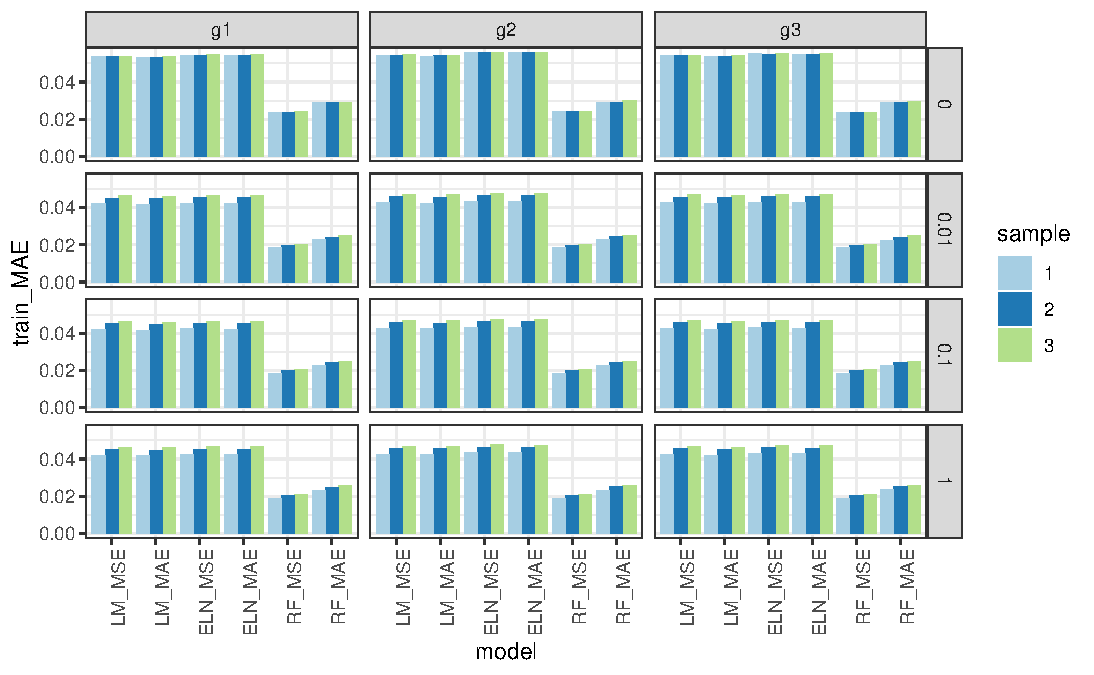
\includegraphics[max size = {\textwidth}{0.5\textheight}]{simulation_train_mae.pdf}
	\caption{Simulation Train MAE}
\end{figure}

\begin{figure}[!htb]
	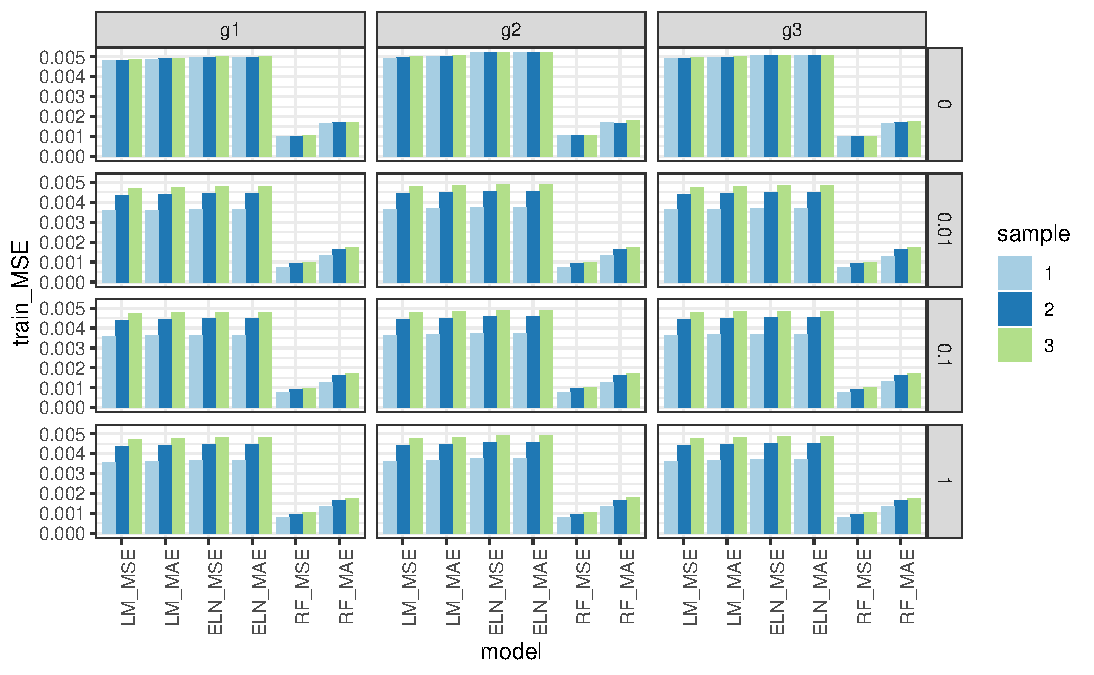
\includegraphics[max size = {\textwidth}{0.5\textheight}]{simulation_train_mse.pdf}
	\caption{Simulation Train MSE}
\end{figure}

\begin{figure}[!htb]
	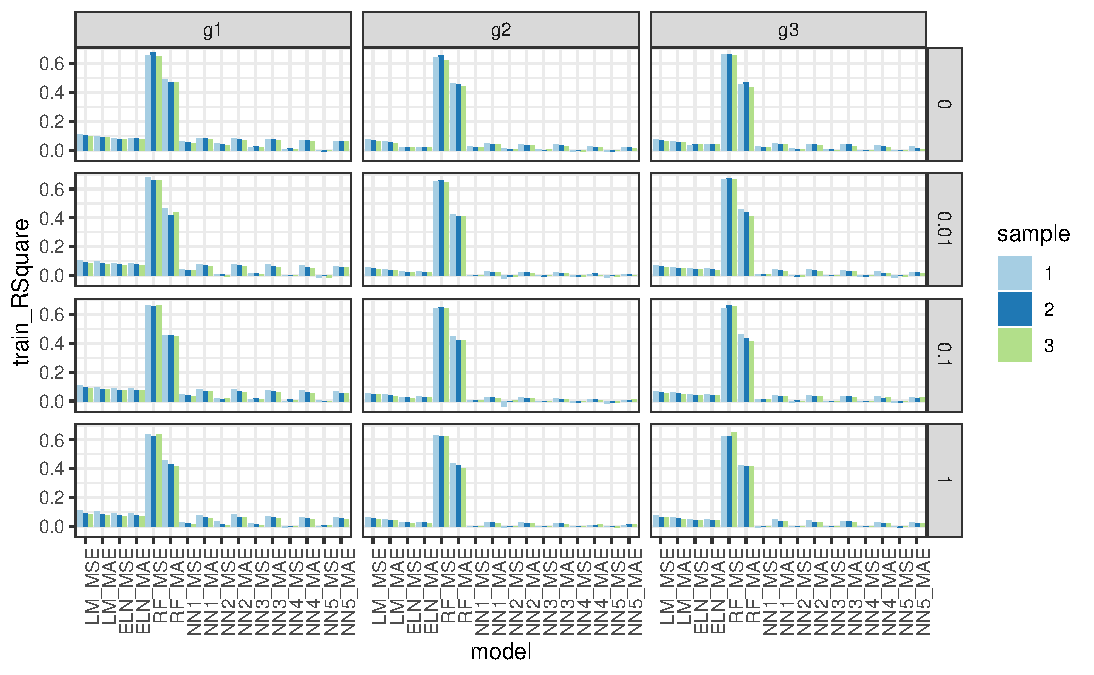
\includegraphics[max size = {\textwidth}{0.5\textheight}]{simulation_train_rsquare.pdf}
	\caption{Simulation Train R Squared}
\end{figure}

\begin{figure}[!htb]
	\begin{center}
		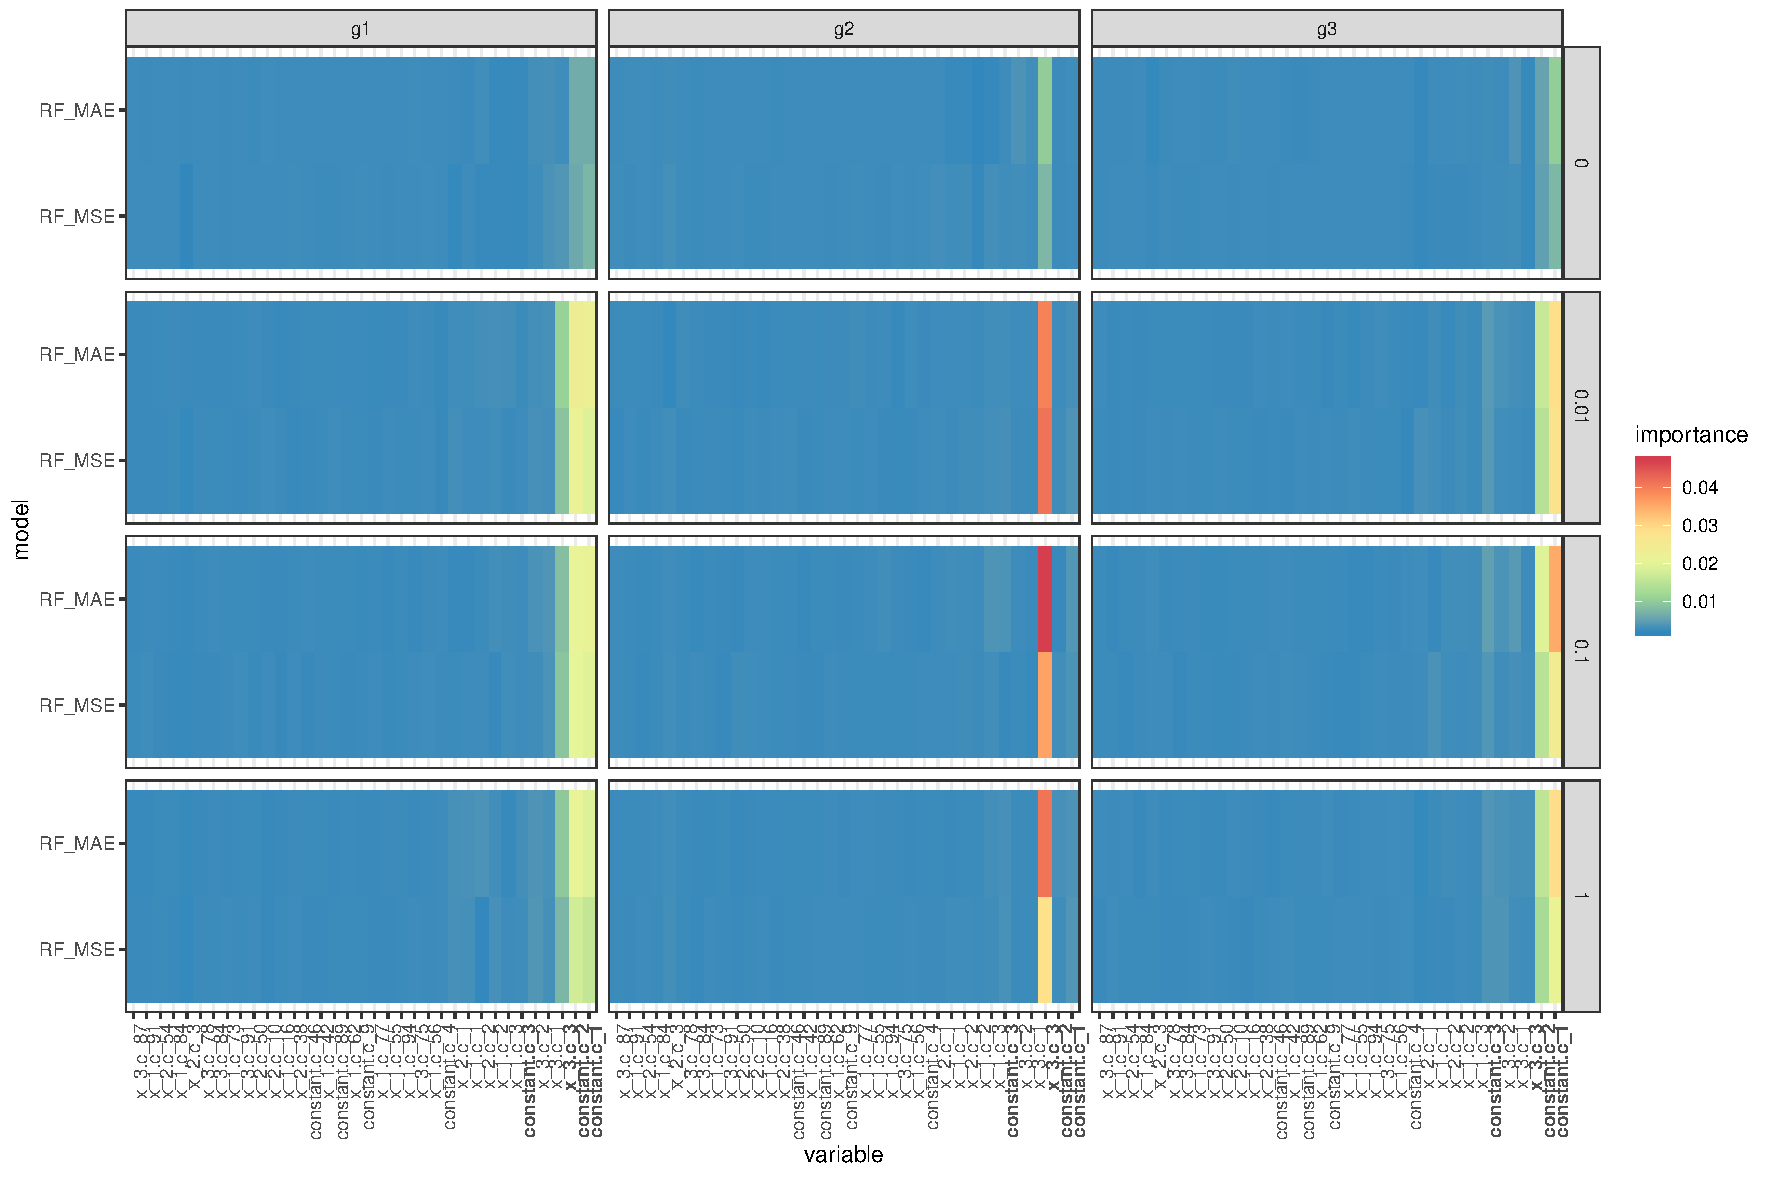
\includegraphics[max size = {\textwidth}{0.5\textheight}]{simulation_ave_vi_plot_pre_rf.pdf}
		\caption{Simulation Variable Importance Plots for Random Forests}
	\end{center}
	\label{fig:rf_sim_vi}
\end{figure}

\begin{figure}[!htb]
	\begin{center}
		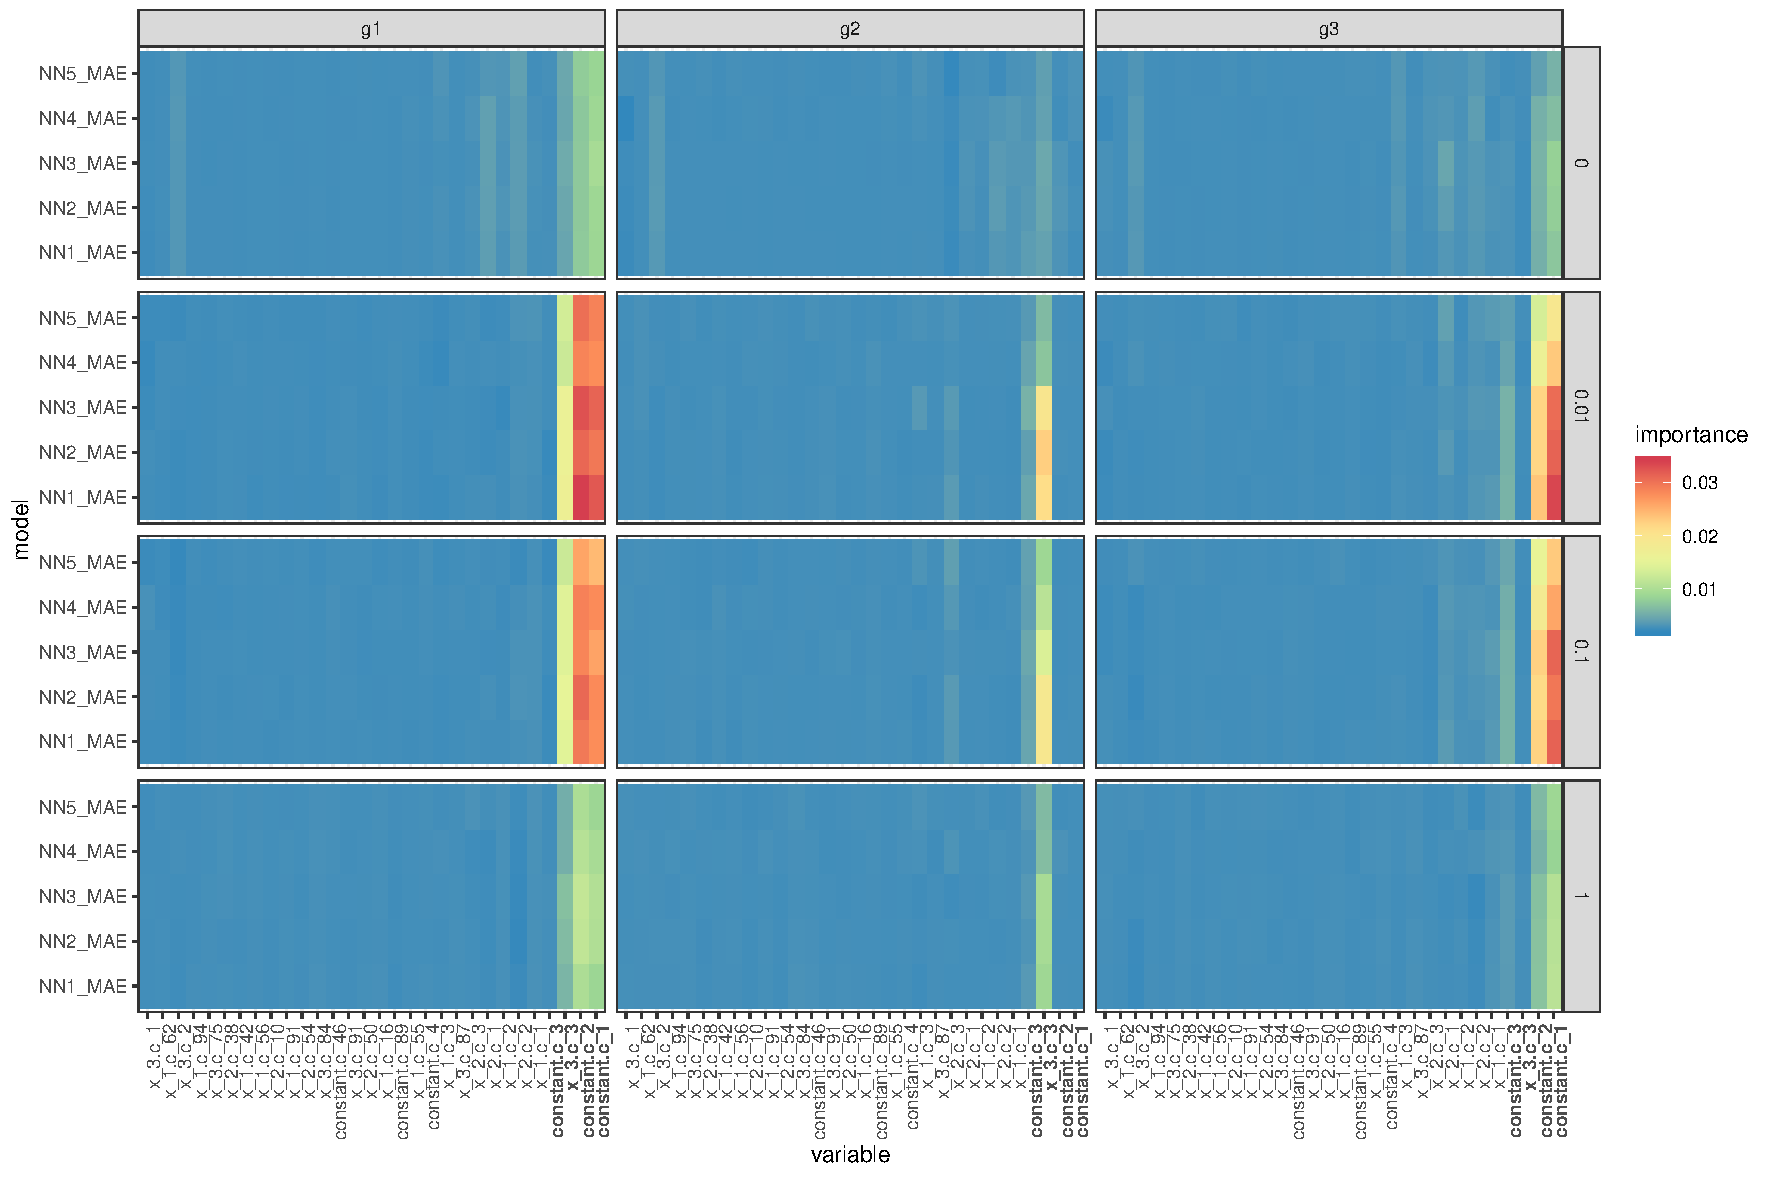
\includegraphics[max size = {\textwidth}{0.5\textheight}]{simulation_ave_vi_plot_pre_nn.pdf}
		\caption{Simulation Variable Importance Plots for Neural Networks}
	\end{center}
	\label{fig:nn_sim_vi}
\end{figure}

%% Hyperparameters

% Penalized Linear Models
\begin{figure}[!htb]
	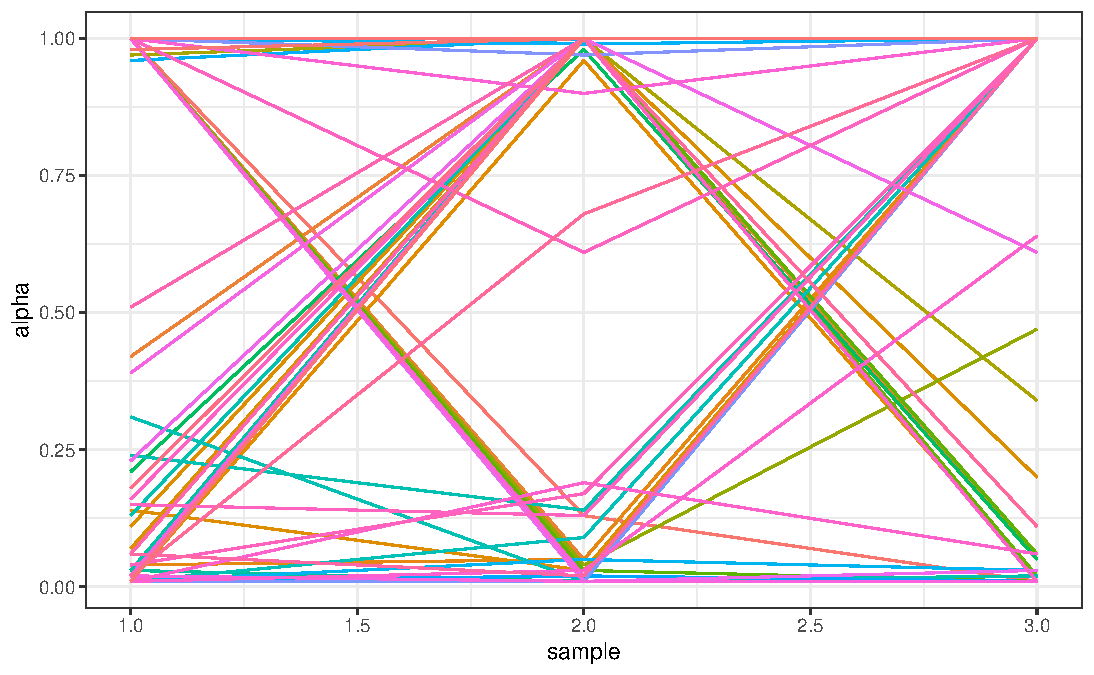
\includegraphics[max size = {\textwidth}{0.4\textheight}]{eln_alpha_plot.pdf}
	\caption{Optimal Alpha Values Across Training Samples for Elastic Net, each colour representing a different simulation realisation}
\end{figure}

\begin{figure}[!htb]
	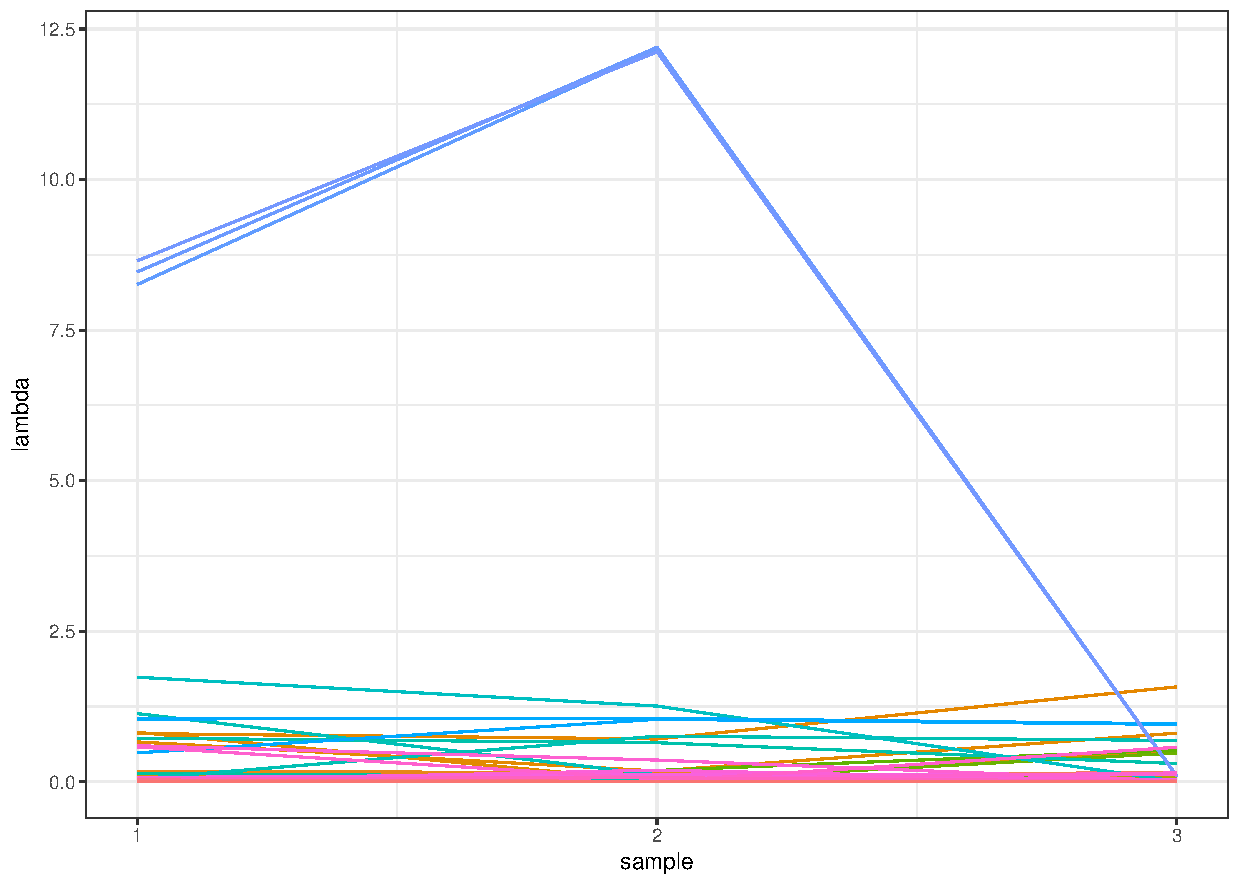
\includegraphics[max size = {\textwidth}{0.4\textheight}]{eln_lambda_plot.pdf}
	\caption{Optimal Lambda Values Across Training Samples for Elastic Net, each colour representing a different simulation realisation}
\end{figure}

% Random Forests

\begin{figure}[!htb]
	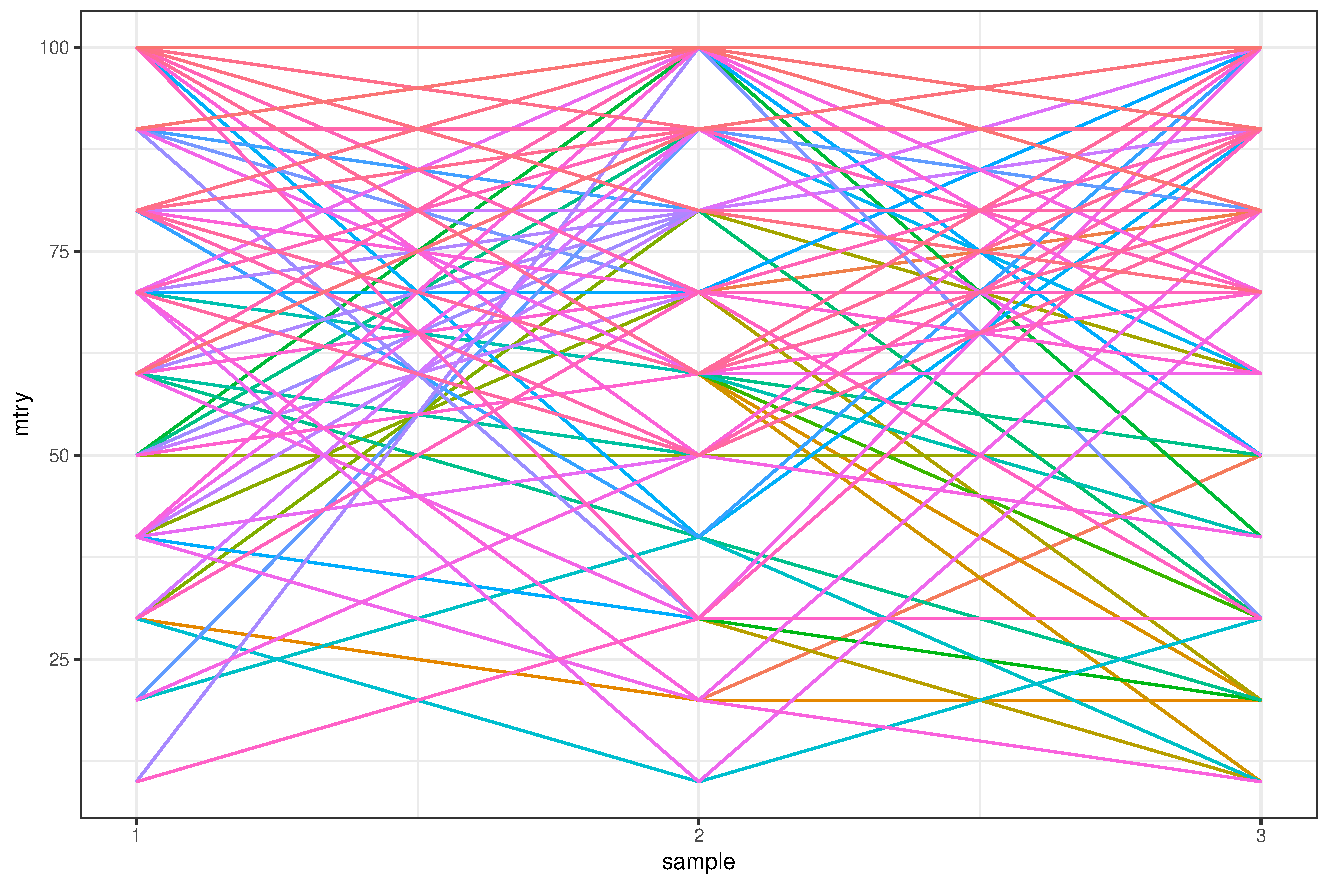
\includegraphics[max size = {\textwidth}{0.4\textheight}]{rf_mtry_plot.pdf}
	\caption{Optimal mtry Values Across Training Samples for Random Forest, each colour representing a different simulation realisation}
\end{figure}

\begin{figure}[!htb]
	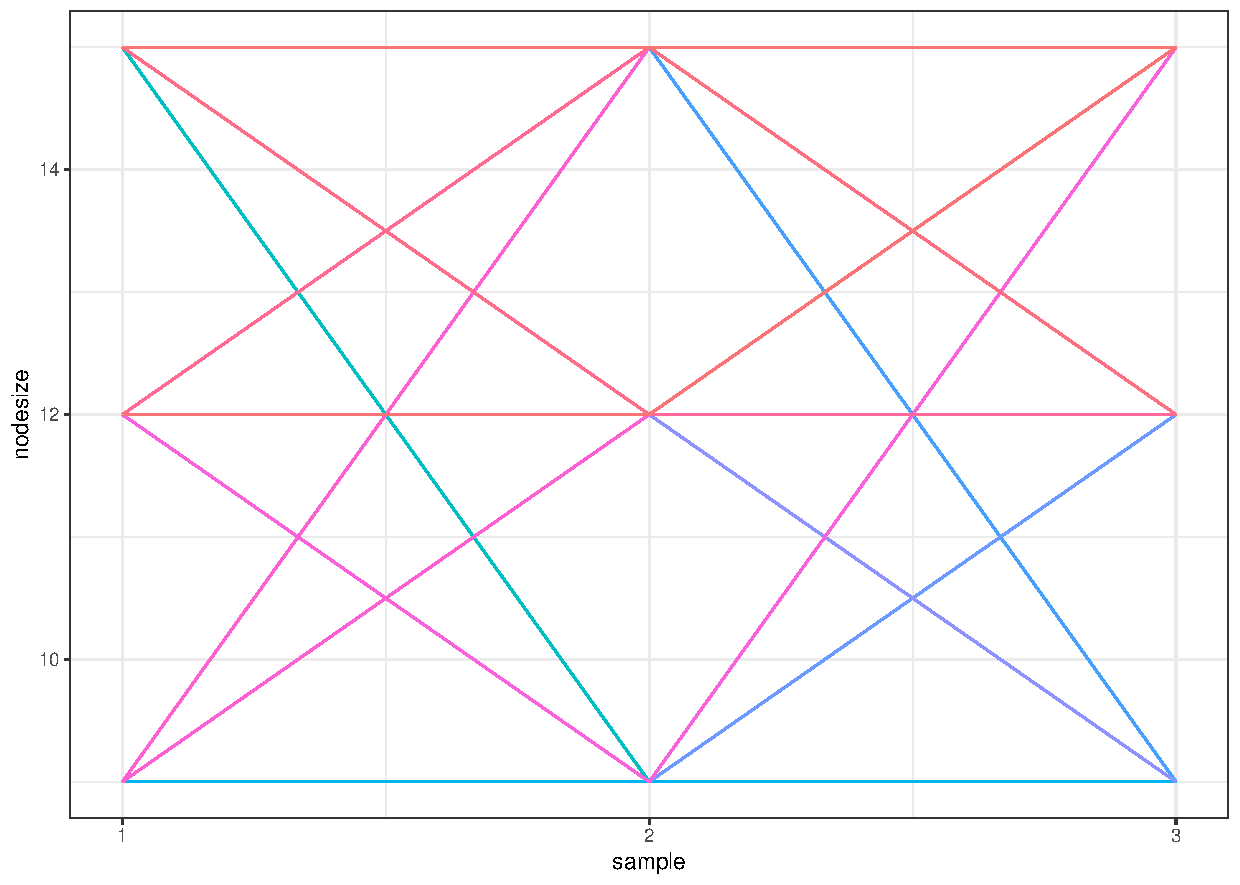
\includegraphics[max size = {\textwidth}{0.4\textheight}]{rf_nodesize_plot.pdf}
	\caption{Optimal nodesize Values Across Training Samples for Random Forest, each colour representing a different simulation realisation}
\end{figure}

\newpage

\subsubsection{Empirical Study}

\begin{figure}[!htb]
	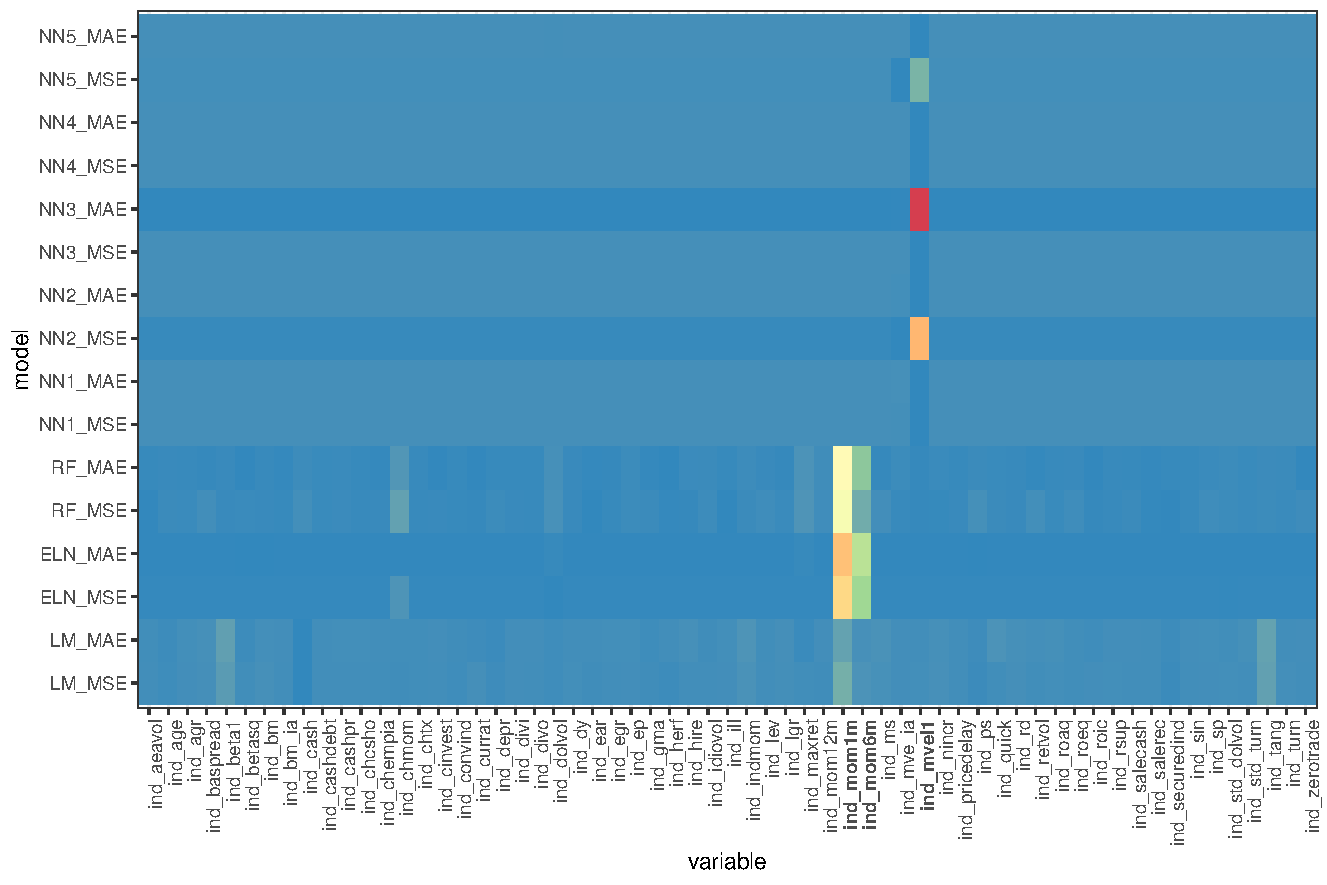
\includegraphics[max size = {\textwidth}{0.5\textheight}]{empirical_sample_1_vi_ind.pdf}
	\caption{Empirical Data Individual Factor Variable Importance for Sample 1}
\end{figure}

\begin{figure}[!htb]
	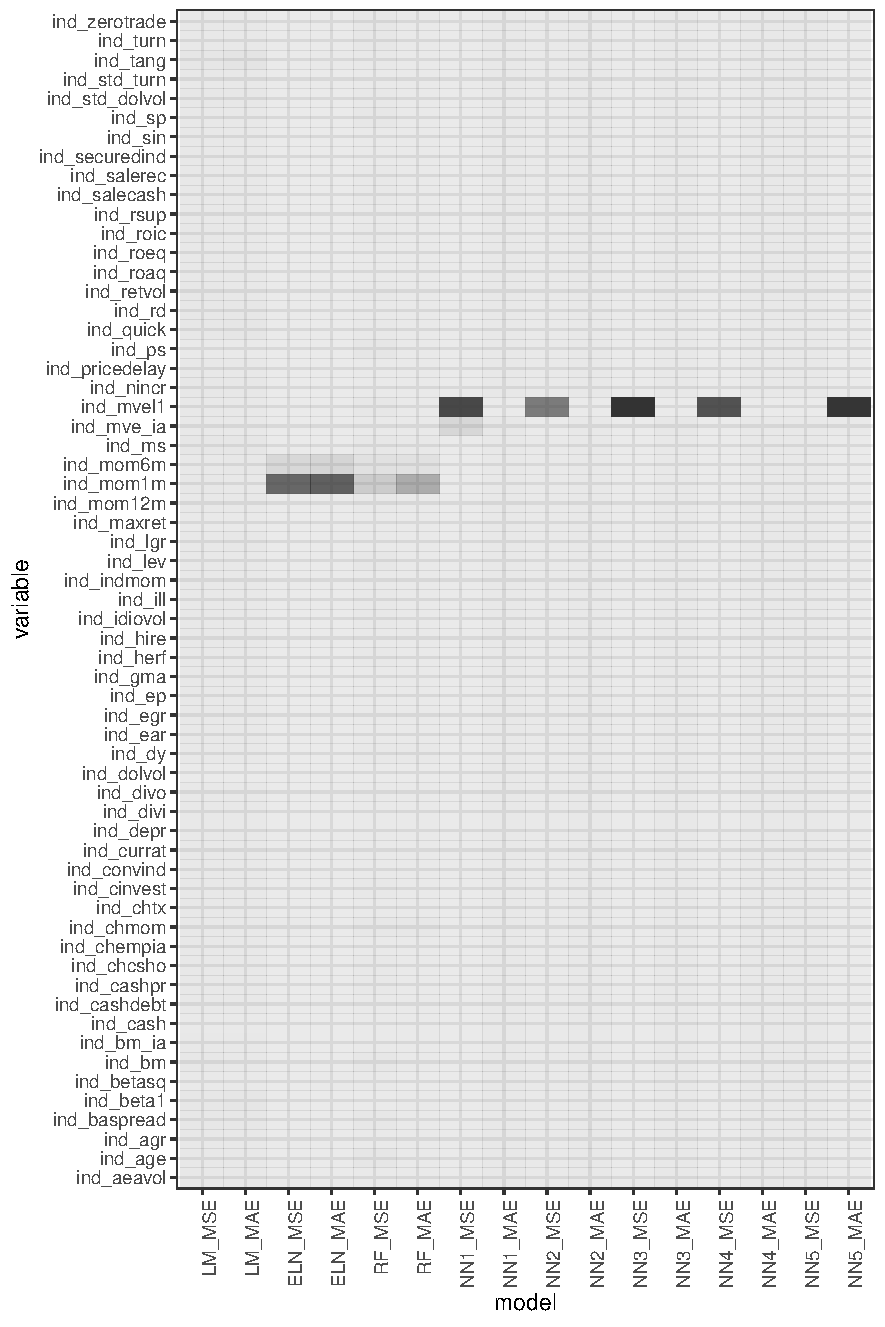
\includegraphics[max size = {\textwidth}{0.5\textheight}]{empirical_sample_2_vi_ind.pdf}
	\caption{Empirical Data Individual Factor Variable Importance for Sample 2}
\end{figure}

\begin{figure}[!htb]
	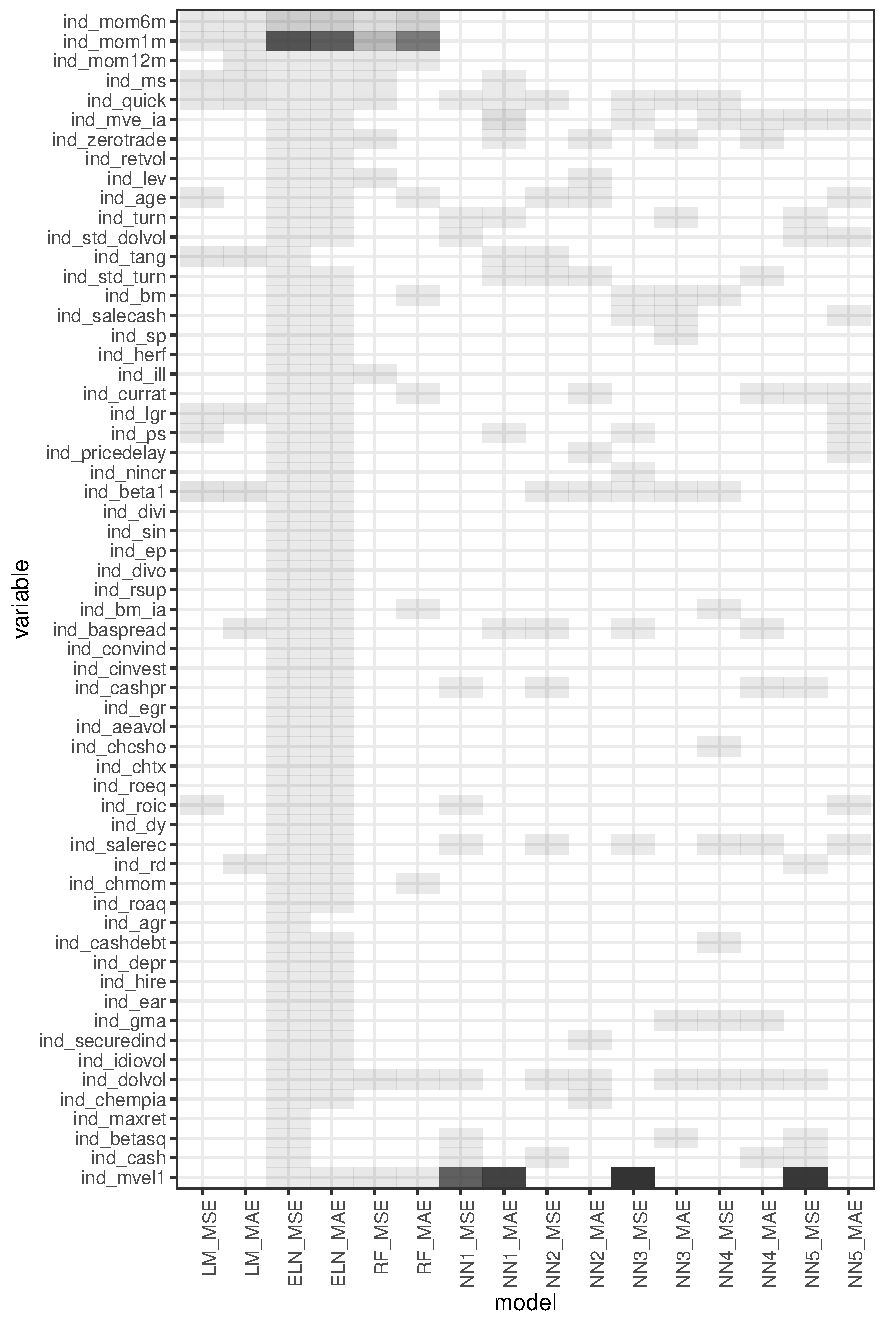
\includegraphics[max size = {\textwidth}{0.5\textheight}]{empirical_sample_3_vi_ind.pdf}
	\caption{Empirical Data Individual Factor Variable Importance for Sample 3}
\end{figure}

\newpage

\subsection{Computational Details}

All computational code is available from:

\url{https://github.com/Meron35/Evaluation-of-Machine-Learning-in-Asset-Pricing}
 
This is a comprehensive repository and contains code for all aspects of this thesis, including simulation code, model fitting, exporting of results, plotting of results, as well as instructions on how to construct and clean the empirical dataset used.  

\subsubsection{Linear Models}

Ordinary Least Squares (OLS) used for fitting with respect to MSE. This is available from many statistical packages, including R's \textbf{stats} package.

The \textbf{quantreg} package which implements quantile linear regression used for fitting linear models with respect to mean absolute error (noting that minimizing 0.5 quantile loss is equivalent to minimizing mae).

\subsubsection{Penalized Linear}

The package \textbf{hqreg} was used to fit penalized regression models with respect to MSE and MAE.

This package efficiently calculates a regularization path of penalization values given a value for $\alpha$. This means that it is much more efficient to instead only supply a grid for $\alpha$, let the algorithm decide its own path of penalization values. The combination of these two parameters which produces the best results on the validation set were then chosen to produce the final model. Note that this is the approach originally suggested by \cite{zou_regularization_2005}.

\subsubsection{Classification and Regression Trees and Random Forests}

The \textbf{randomforestSRC} package was used to fit both random forests for mean regression and quantile regression.

To maintain computational feasibility, all random forest models were grown using 50 trees, and their \textit{mtry} \textit{nodesize} hyperparameters tuned. These correspond to the number of predictors included for each tree, and the depth of each tree respectively. 

Rather than use the randomly determined out of bag (OOB) observations for hyperparameter tuning, we explicitly use a separate validation set that is closer to the test set in time, in order to maintain temporal ordering of the data.

For full details of the classification and regression tree algorithms see \cite{breiman_classification_1984}. 

For full details of the Random Forest algorithm see \cite{breiman_random_2001}. 

\subsubsection{Neural Networks}

Nueral Networks were fit using the \textbf{keras} package, using the \textbf{tensorflow} backend. 

Due to computational limitations, a systematic grid search or random search approach for hyperparameters was not feasible. Instead, common hyperparameters that are usually grid searched were tuned manually. 

\begin{table}[!htb]
	\begin{tabular}{|lll|}
		\hline
		Hyperparameter & Options Considered & Optimal Choice \\ \hline
		Activation Function & ReLU, Leaky ReLU, tanh & tanh \\
		Optimizer & ADAM, NADAM, SGD, RMSPROP & ADAM \\
		Learning Rate & (0.1, 0.01, 0.001, 0.0001) & 0.001 \\
		L1 Penalty & (1, 0.1, 0.01, 0.001) & 0.01 \\
		Batch Size & (32, 64, 128, 256, 512, 1024, 2048) & 256 (Empirical), 128 (Simulated) \\
		Early Stopping Patience & (10, 20, 30, 40, 50) & 40 \\ \hline
	\end{tabular}
	\caption{Hyperparameters Considered for Neural Networks}
\end{table}

For full details of the ADAM optimizer see \cite{kingma_adam:_2014}.

For full details of the Batch Normalization Algorithm see \cite{ioffe_batch_2015}.

We present the algorithm implemented for early stopping of training. Note that this corresponds to \textit{restore\_best\_weights = TRUE} in \textbf{keras}'s implementation.

\begin{algorithm}[!htb]
	\SetAlgoLined
	Initialize $j = 0$, $\epsilon = \infty$ and select the patience parameter $p$ (max iterations)\
	
	\While{j < p}{
		Update $\theta$ using the training algorithm\
		Calculate the prediction error from the validation sample, denoted as \(\epsilon'\)\
		
		\eIf{\(\epsilon' < \epsilon\)}
		{\(j \leftarrow 0\)\
			
			\(\epsilon \leftarrow \epsilon'\)\
			
			\(\theta' \leftarrow \theta\)}
		{\(j \leftarrow j+1\)}
	}
	\KwResult{$\theta'$ is the final parameter estimate}
	\caption{Early stopping via validation}
\end{algorithm}

\subsubsection{Tuning of Simulated Datasets}

The simulated datasets were tuned according to the following statistics: average individual time series R squared, average annualized volatility, and cross sectional R squared, and true/predictive R squared.

The methodology for evaluating average time series R squared and cross sectional R squared is consistent with that detailed by \cite{cochrane_asset_2005}. The steps are reproduced here for reference; for complete details refer to \cite{cochrane_asset_2005}.

First evaluate the following OLS model:

\begin{equation}
	R_{it} = a_i + \beta_i' f_{it} + \epsilon_{it} 
\end{equation}

where $f_{it}$ represents the \textit{true} factors in the returns process. The corresponding R-squared value for this time series regression is calculated across all stocks and averaged to yield the average time series R-Squared. 

A cross sectional regression for the risk premia is then run across assets of average returns on the factor coefficients:

\begin{equation}
	\bar{R_{it}} = \alpha_i = \beta_i' \lambda
\end{equation}

where the $\beta_i'$ are the estimated coefficients from each time series regressions run previously. The corresponding R squared for this regression is the cross sectional R squared.

The true R squared is a measure of signal to noise ratio i.e. how much of the returns data is due to 
This is simply calculated by running a pooled ordinary least squares regression on the entire panel, using the underlying g() as the "predictions.' The resulting R squared value is therefore a measure of how much of the panel can be explained by the g() term exclusive of any noise or error terms.

%%%%%%%%%%%%%%%%%%%%%%%%%%%%%%%%%%
%%BIBLIOGRAPHY
%%%%%%%%%%%%%%%%%%%%%%%%%%%%%%%%%%

\bibliographystyle{jfe}
\bibliography{Bibliography}

\end{document}